\documentclass[11pt]{article}
\usepackage[margin=1.4in]{geometry}
\usepackage[brazil]{babel}
\usepackage[utf8]{inputenc}
\usepackage{amsmath}
\usepackage{indentfirst}
\usepackage{cite}
\usepackage{url}
\usepackage{graphics}
\usepackage{graphicx}
\usepackage{caption}
\usepackage{subcaption}
\usepackage{multirow}
\usepackage{amsfonts}

\title{Geração de Malhas\\Poligonização}
\author{Rafael Umino Nakanishi}

\date{}

\begin{document}
	\maketitle
	\section{Objetivo} % (fold)
	\label{sec:objetivo}
		O objetivo desse trabalho foi implementar o método \emph{Marching Tetrahedra} para geração de malhas a partir de superfícies implícitas. O método foi inicialmente proposto por Bloomenthal \cite{bloomenthal1994implicit} e tem como base a técnica \emph{Marching Cubes}\cite{lorensen1987marching}. A principal vantagem da técnica de Bloomenthal é a não presença de ambiguidades gerada pelos cubos no momento da detecção da superfície.

		Nas seções seguintes discutiremos brevemente sobre a técnica e os detalhes de implementação bem como a estrutura escolhida para armazenamento da malha. Por fim apresentamos alguns resultados obtidos utilizando equações implícitas de superfícies conhecidas.
	% section objetivo (end)

	\section{Poligonização} % (fold)
		Nas subseções seguintes faremos uma breve descrição dos métodos implementados para poligonalizar uma superfície implícita. Ao aplicarmos técnica \emph{Marching Tetrahedra} obtemos uma triangulação inicial do modelo, que como poderá ser visto nas Seção \ref{sec:resultados} apresenta triângulos com qualidade muito inferior. Para contornarmos esse problema, aplicamos uma técnica de suavização para melhorar seu aspecto.

		\subsection{Marching Tetrahedra}
		\label{sec:marching}
			O método de \emph{Marching Tetrahedra} avalia o valor da função implícita em todos os pontos de um tetraedro para detectar intersecções com a superfície que se deseja renderizar. Pela Figura \ref{fig:tetras} é possível visualizar os possíveis pontos de intersecção com a superfície. Se os sinais obtidos em cada ponto são diferentes, então, pelo Teorema do Valor Intermediário, pode-se dizer que o zero da função encontra-se entre os dois pontos com sinais opostos. A partir disso, podemos criar um conjunto de triângulos que descreverão a superfície implícita, onde os pontos que são os zeros da função encontrados serão vértices da malha.

			\begin{figure}
				\centering
				\begin{subfigure}[b]{0.3\textwidth}
					\centering
					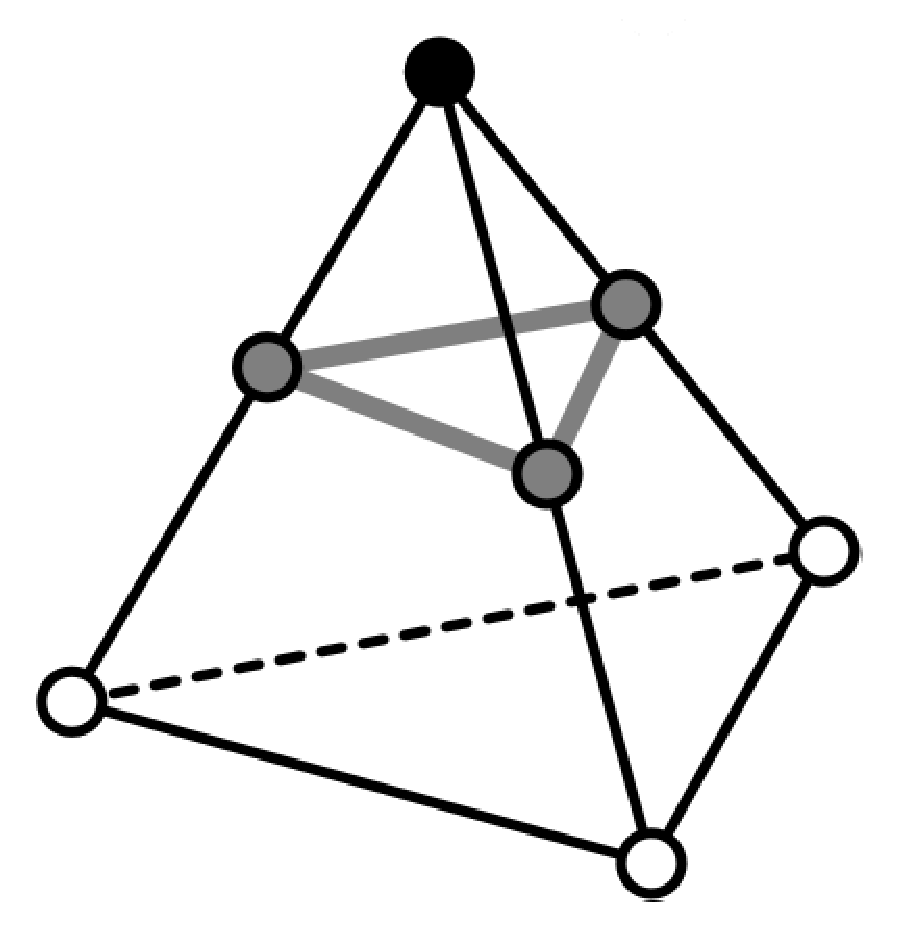
\includegraphics[height=4cm]{figures/tetra01}
				\end{subfigure}
				\begin{subfigure}[b]{0.3\textwidth}
					\centering
					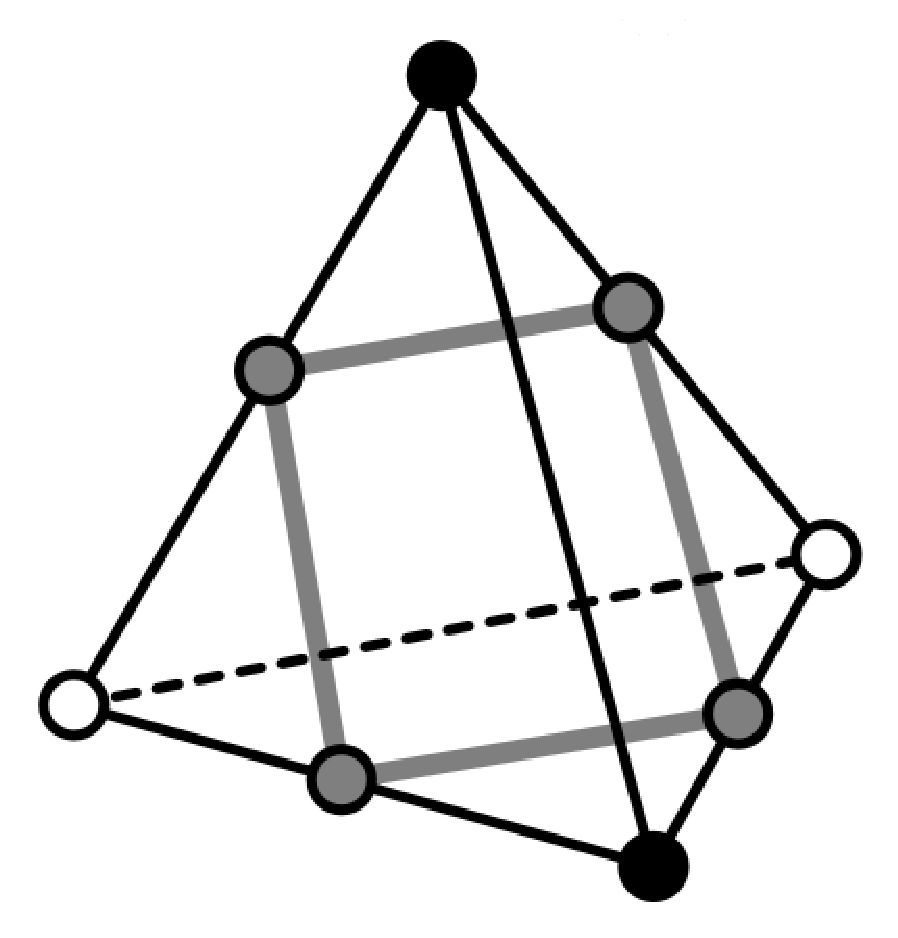
\includegraphics[height=4cm]{figures/tetra02}
				\end{subfigure}
				\begin{subfigure}[b]{0.3\textwidth}
					\centering
					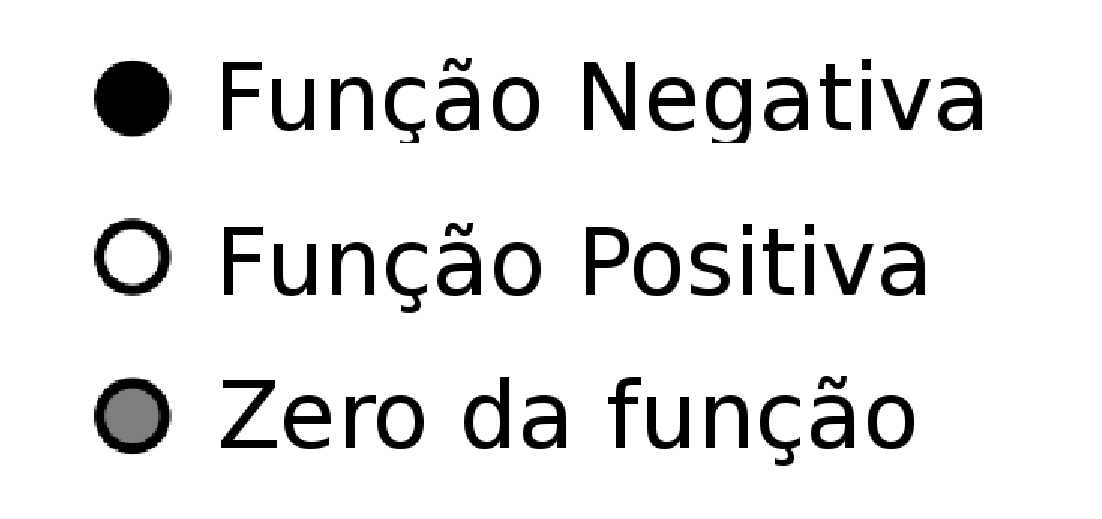
\includegraphics[height=2cm]{figures/tetra03}
				\end{subfigure}
				\caption{Dois possíveis casos de intersecção com a superfície, a menos de rotações. No caso em que a intersecção resulta em um quadrilátero, basta dividi-lo na diagonal para se obter uma malha apenas de triângulos}
				\label{fig:tetras}
			\end{figure}
		% section marching (end)
		\subsection{Suavização} % (fold)
		\label{sub:suavizacao}
			A suavização aplicada é descrita por Botsch e Kobbelt \cite{botsch2004}. Ela é baseada em mover um vértice para o baricentro do seu 1-anel, como é ilustrado na Figura \ref{fig:baricentro}. Dessa forma a qualidade dos triãngulos ao longo da suavização é melhorada.

			\begin{figure}[h]
				\centering
				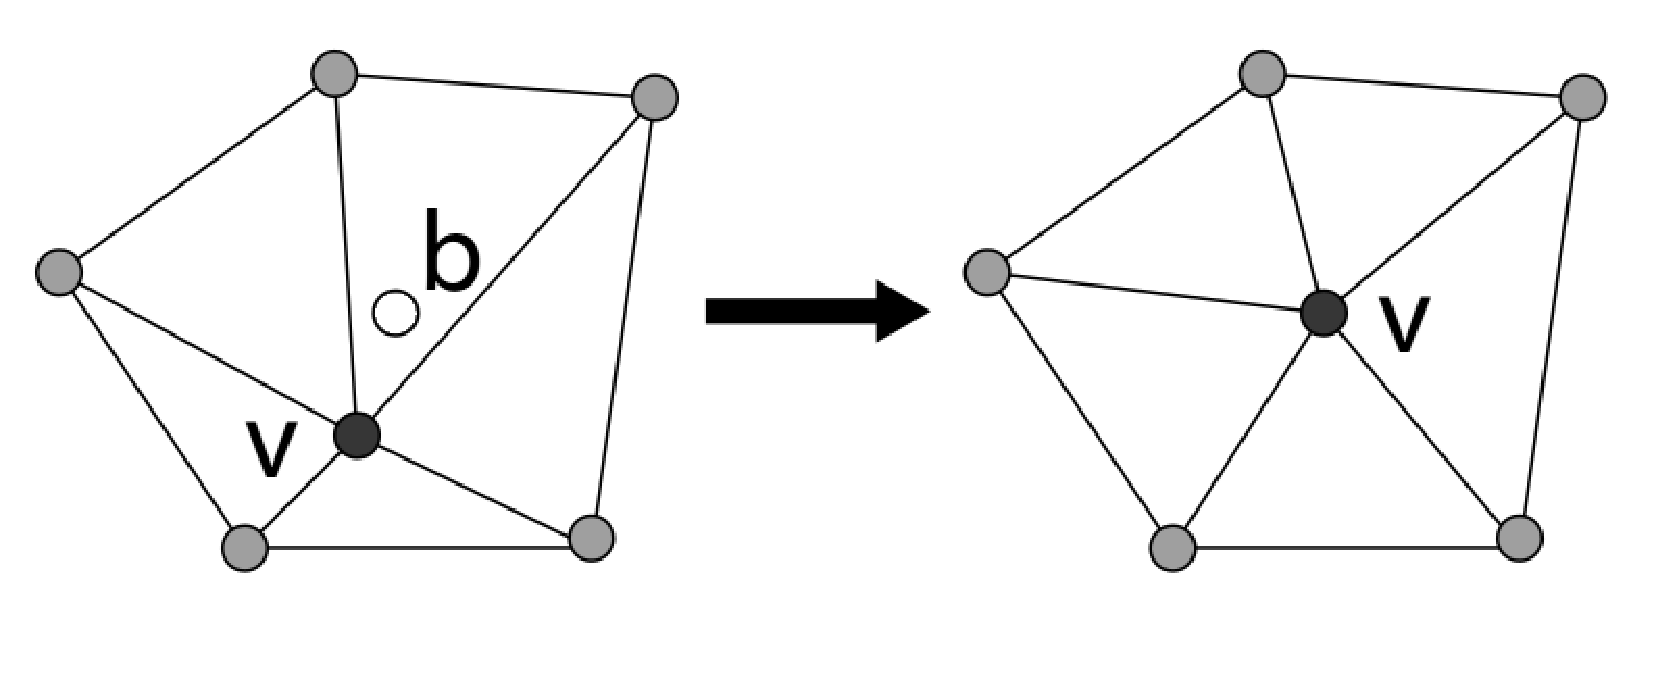
\includegraphics[height=3cm]{figures/baricentro.eps}
				\caption{Ilustração do deslocamento de um vértice para o baricentro do seu 1-anel}
				\label{fig:baricentro}
			\end{figure}

			A posição do novo vértice pode ser descrita como $$ \mathbf{v} = \mathbf{v} + \alpha (\mathbf{d_v} - (\mathbf{d_v} \cdot \mathbf{n_v})\mathbf{n_v} )$$, em que $\mathbf{n_v}$ é a normal do vértice, $\alpha$ é um fator de relaxação, $\alpha \in [0,1]$, e $\mathbf{d_v} = \mathbf{b_v} - \mathbf{v}$ é o vetor deslocamento entre a posição atual do vértice e o baricentro.
			
		% subsection suavizacao (end)

	\section{Detalhes de Implementação} % (fold)
	\label{sec:detalhes}
		Nessa seção discutiremos alguns detalhes pertinentes da técnica, que valem ser ressaltados. Entre eles, podemos destacar a estrutura de dados que foi utilizada, bem como o método aplicado para se encontrar os tetraedros que interceptam a superfície implícita.

		\subsection{Estrutura de dados} % (fold)
		\label{sub:estrutura}
			A estrutura de dados utilizadas para a implementação do método foi a matriz de adjacência. Tal estrutura permite o armazenamento dos vizinhos de cada vértice, o torna a implementação da suavização mais agradável e prática.

			Podemos descrever uma matriz de adjacência como sendo uma matriz na qual as linhas representam os vértices e nas colunas a existência de vizinhança com outro vértice. Um exemplo gráfico pode ser visto na Figura \ref{fig:adjmatrix}. Note nesse mesmo exemplo que o 1-anel do vértice é facilmente recuperado fazendo um acesso apenas à linha que o representa.

			\begin{figure}[h]
				\includegraphics[height=4cm]{figures/adjmatrix}
				\caption{Triangulação com sua respectiva matriz de adjacência}
				\label{fig:adjmatrix}
			\end{figure}
		% subsection estrutura (end)
		
		\subsection{Decomposição do cubo} % (fold)
		\label{sub:decomposicao}
			Inicialmente, para busca dos vértices que fazem parte da superfície criamos uma caixa que a envolve com segurança (Figura \ref{fig:boundingbox}. Dessa forma, subdividimos tal caixa por caixinhas menores, que serão responsáveis por detectar intersecção com a superfície.
			A deteção é feita olhando-se o sinal em cada vértice dos mini-cubos. Caso haja algum vértice cujo sinal seja diferente dos demais, é aplicado uma decomposição em tetraedros. 

			\begin{figure}[h]
				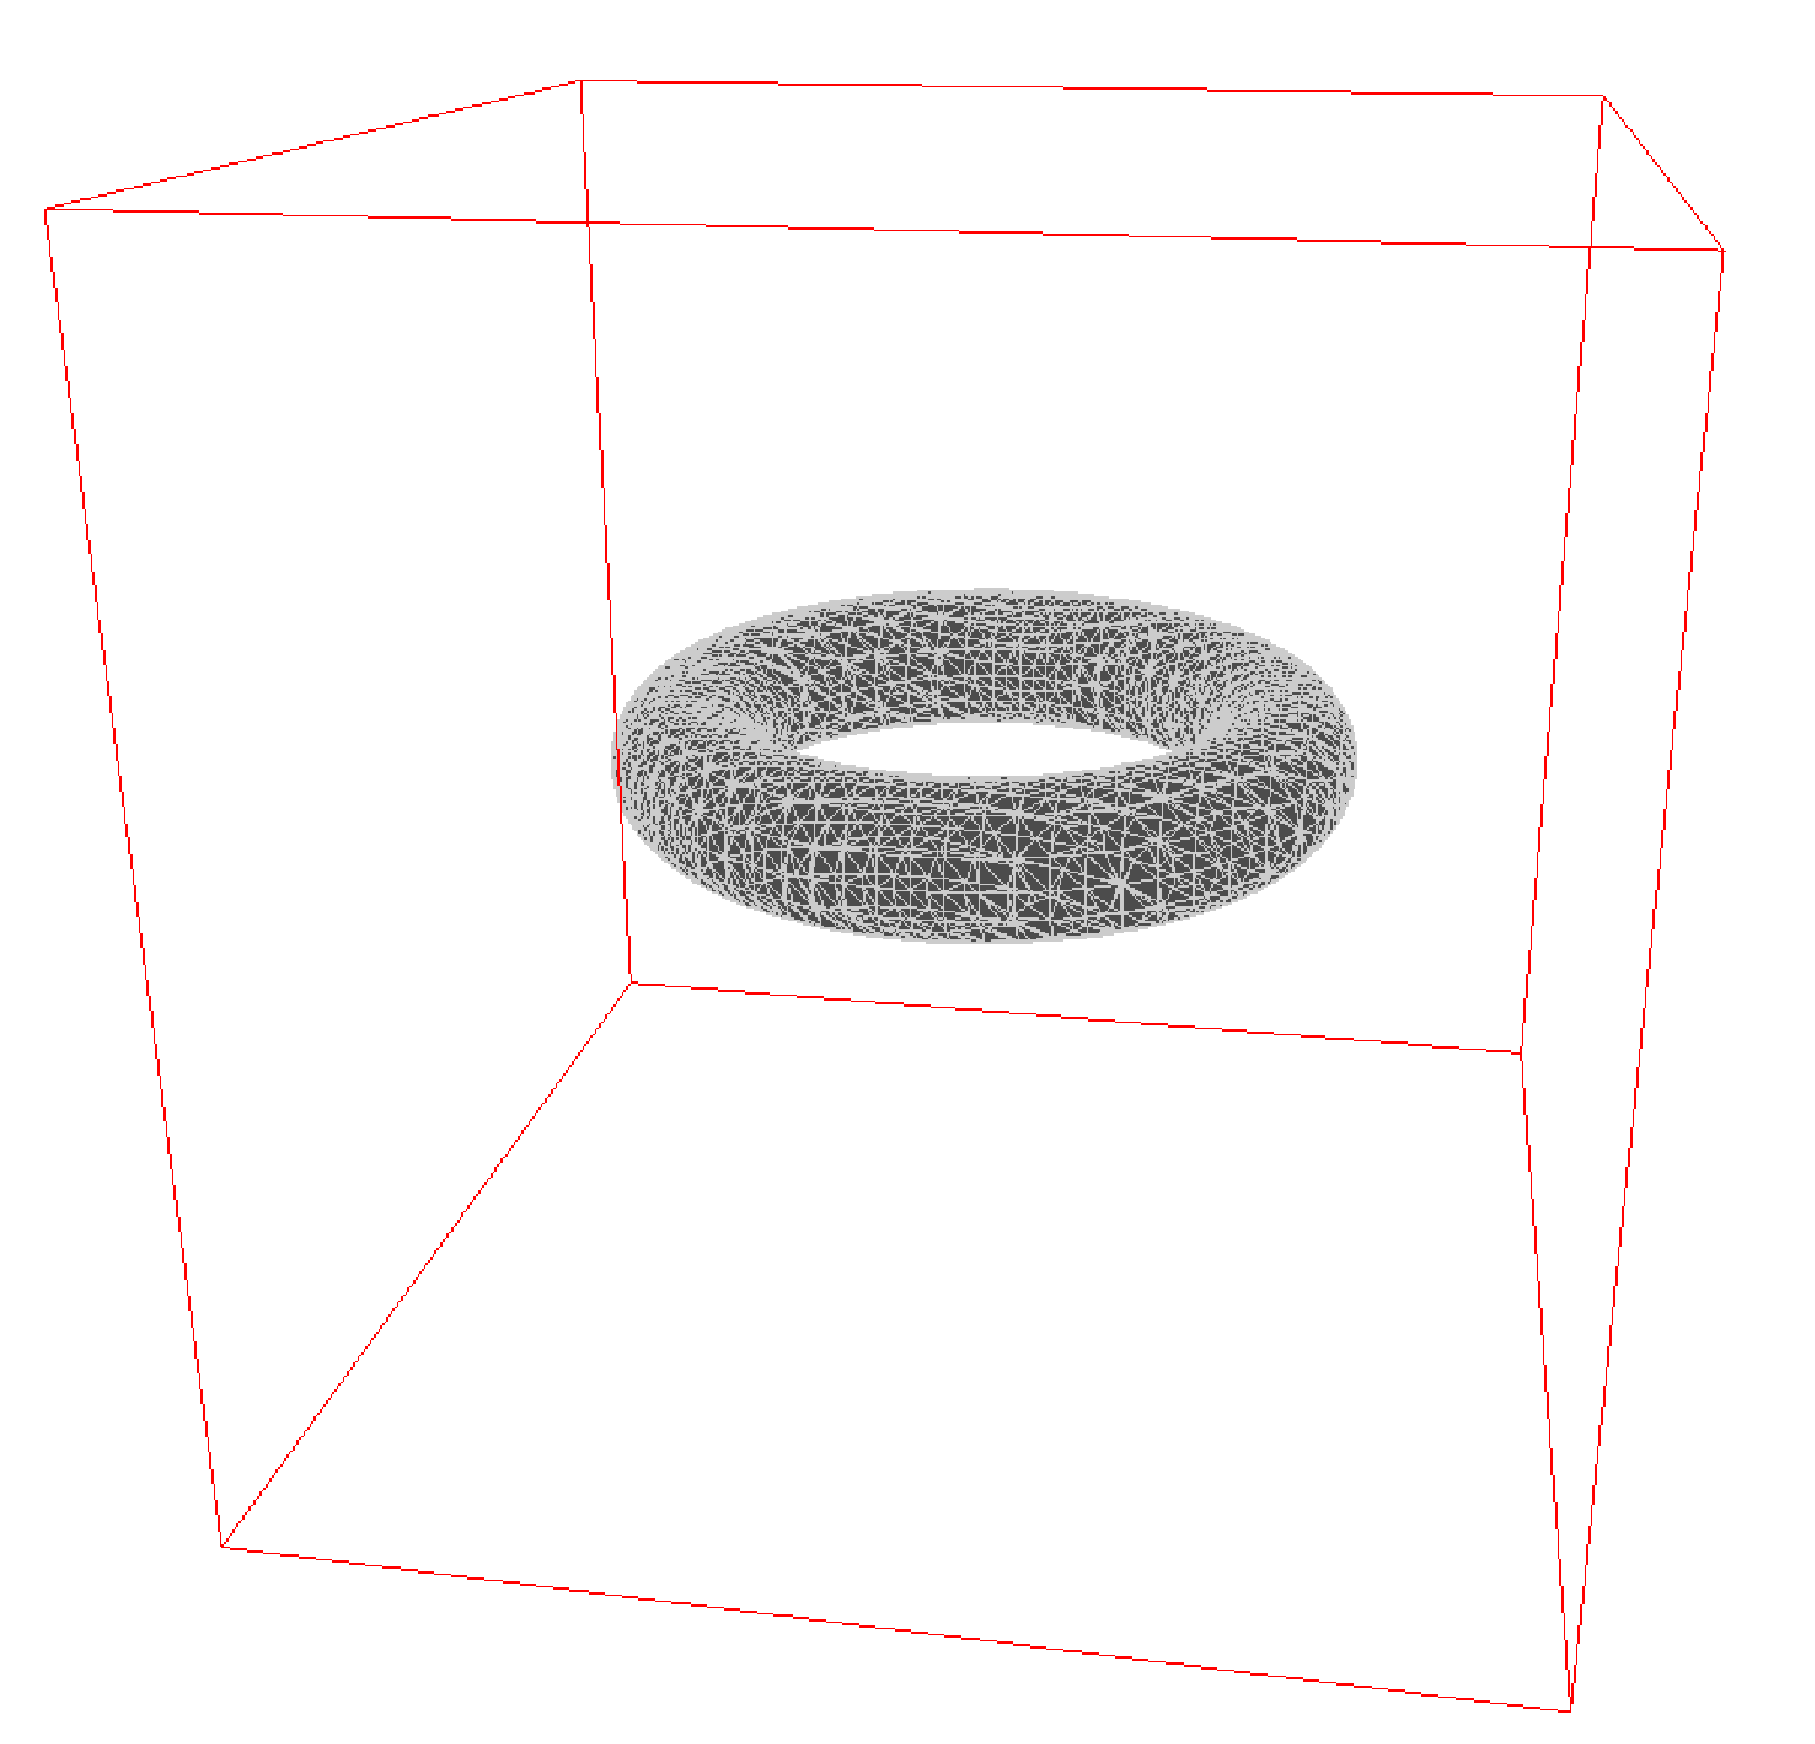
\includegraphics[height=4cm]{figures/boundingbox}
				\caption{Caixa de segurança utilizada. Tal caixa é decomposta em mini-cubos que serão utilizados para se encontrar intersecções com a superfície implícita}
			\end{figure}

			Indexando cada vértice como mostrado na Figura \ref{fig:cubetotetra}, podemos decompor cada cubo em seis tetraedros. Para cada tetraedro decomposto, novamente é aplicado o teste de intersecção e em caso positivo, procura-se pelo zero da função e então constroi-se a triangulação para a malha.

			\begin{figure}[h]
				\includegraphics[height=4cm]{figures/decomposition}
				\caption{Decomposição do cubo em seis tetraedros}
				\label{fig:cubetotetra}
			\end{figure}
		% subsection decomposicao (end)

	% section detalhes (end)

	\section{Resultados} % (fold)
	\label{sec:resultados}
		Apresentamos nessa seção alguns resultados obtidos a partir da execução da técnica implementada.

		As superfícies que utilizamos como funções implícitas são bem conhecidas: esfera e toro e suas respectivas equações podem ser vistas nas Equações \ref{eq:sphere} e \ref{eq:torus}. Nas equações, $R$ é definido como o raio da esfera e raio externo do toro, enquanto $r$ é definido como o raio interno do toro.

		\begin{eqnarray}
			x^2 + y^2 + z^2 -R &\text{\qquad Equação da Esfera} \label{eq:sphere}\\
			(x^2 + y^2 +z^2 + R^2 - r^2)^2 - 4(x^2 + y^2) &\text{\qquad Equação do Toro} \label{eq:torus}
		\end{eqnarray}

		Podemos ver nas Figuras \ref{fig:mesh:sphere} e \ref{fig:mesh:torus} que a malha original é dada com vários triângulos ruins, gerados a partir do algoritmo de \emph{Marching Tetrahedra}. Com a aplicação da suavização, a qualidade visual dos triângulos foi aumentando. Essa melhora visual é comprovada através dos histogramas de qualidade apresentados nas Figuras \ref{fig:hist:sphere} e \ref{fig:hist:torus}. Podemos ver que, inicialmente, muitos triângulos possuiam qualidade inferior a 0.5. Tal índice diminui com o passar das iterações, chegando à convergência.

		\begin{figure}
			\centering
			\begin{subfigure}[b]{0.45\textwidth}
				\centering
				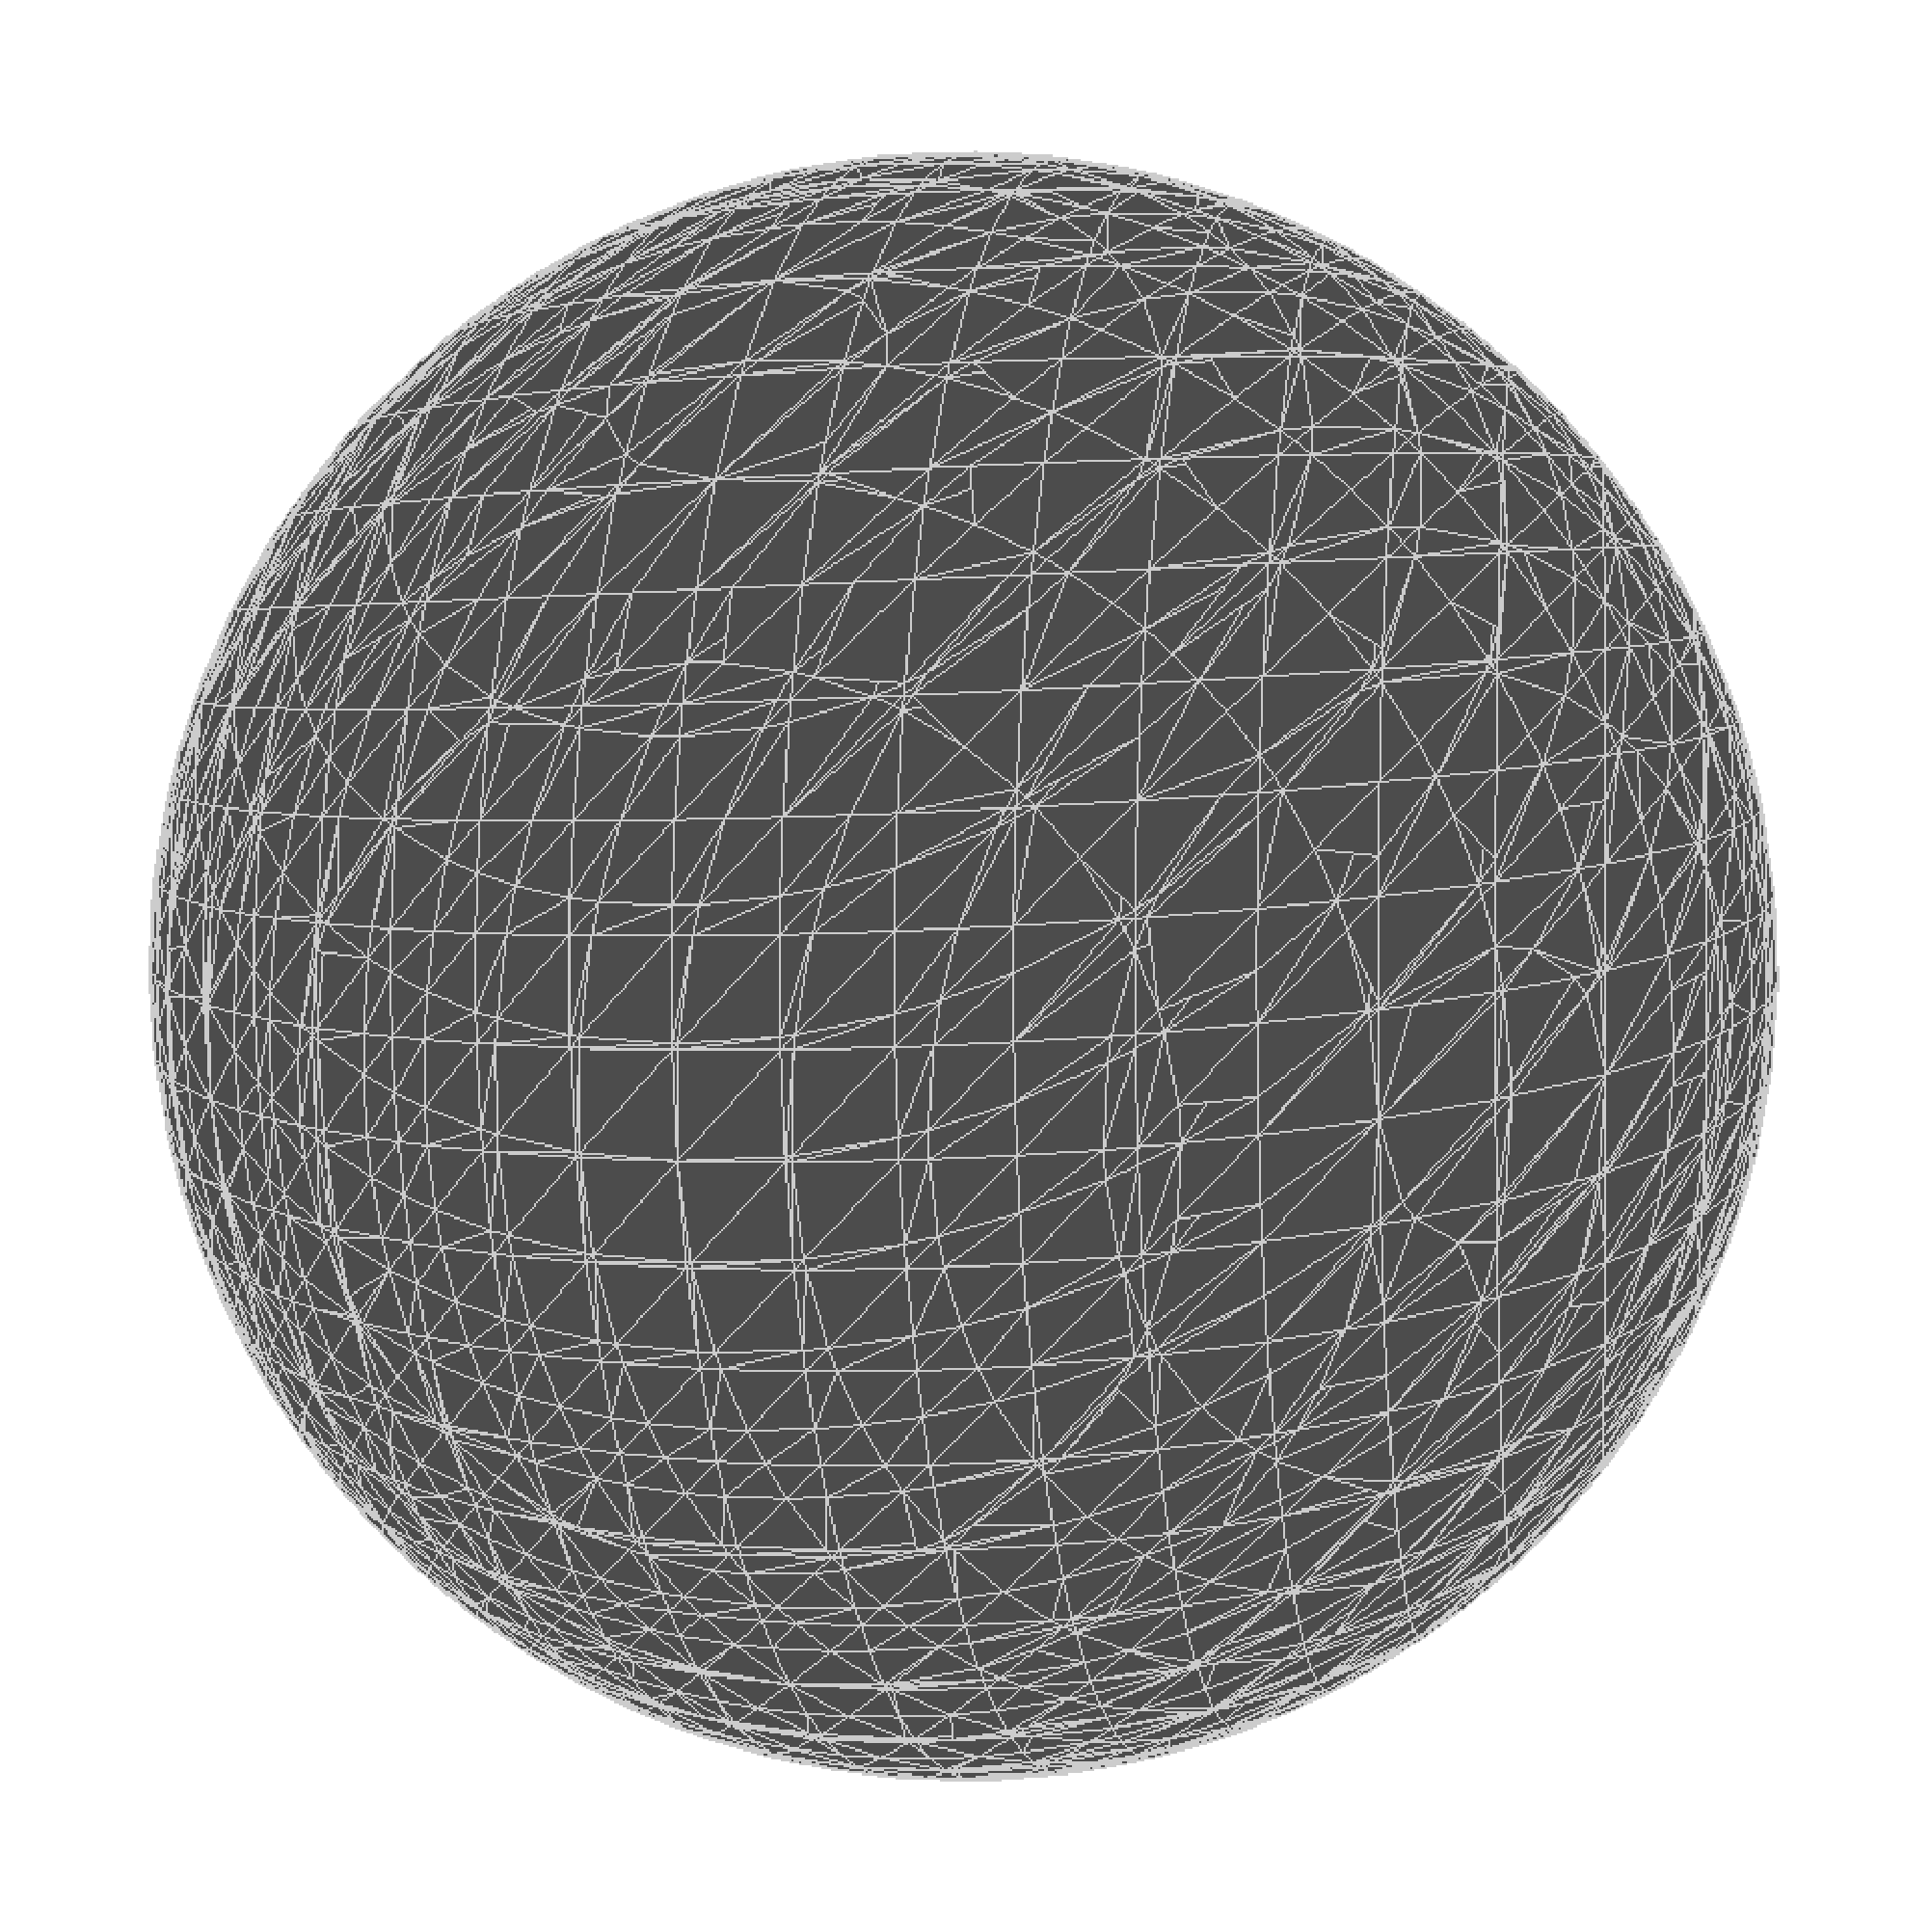
\includegraphics[width=\textwidth]{figures/0iter_sphere_mesh}
				\caption{Malha inicial}				
			\end{subfigure}
			\begin{subfigure}[b]{0.45\textwidth}
				\centering
				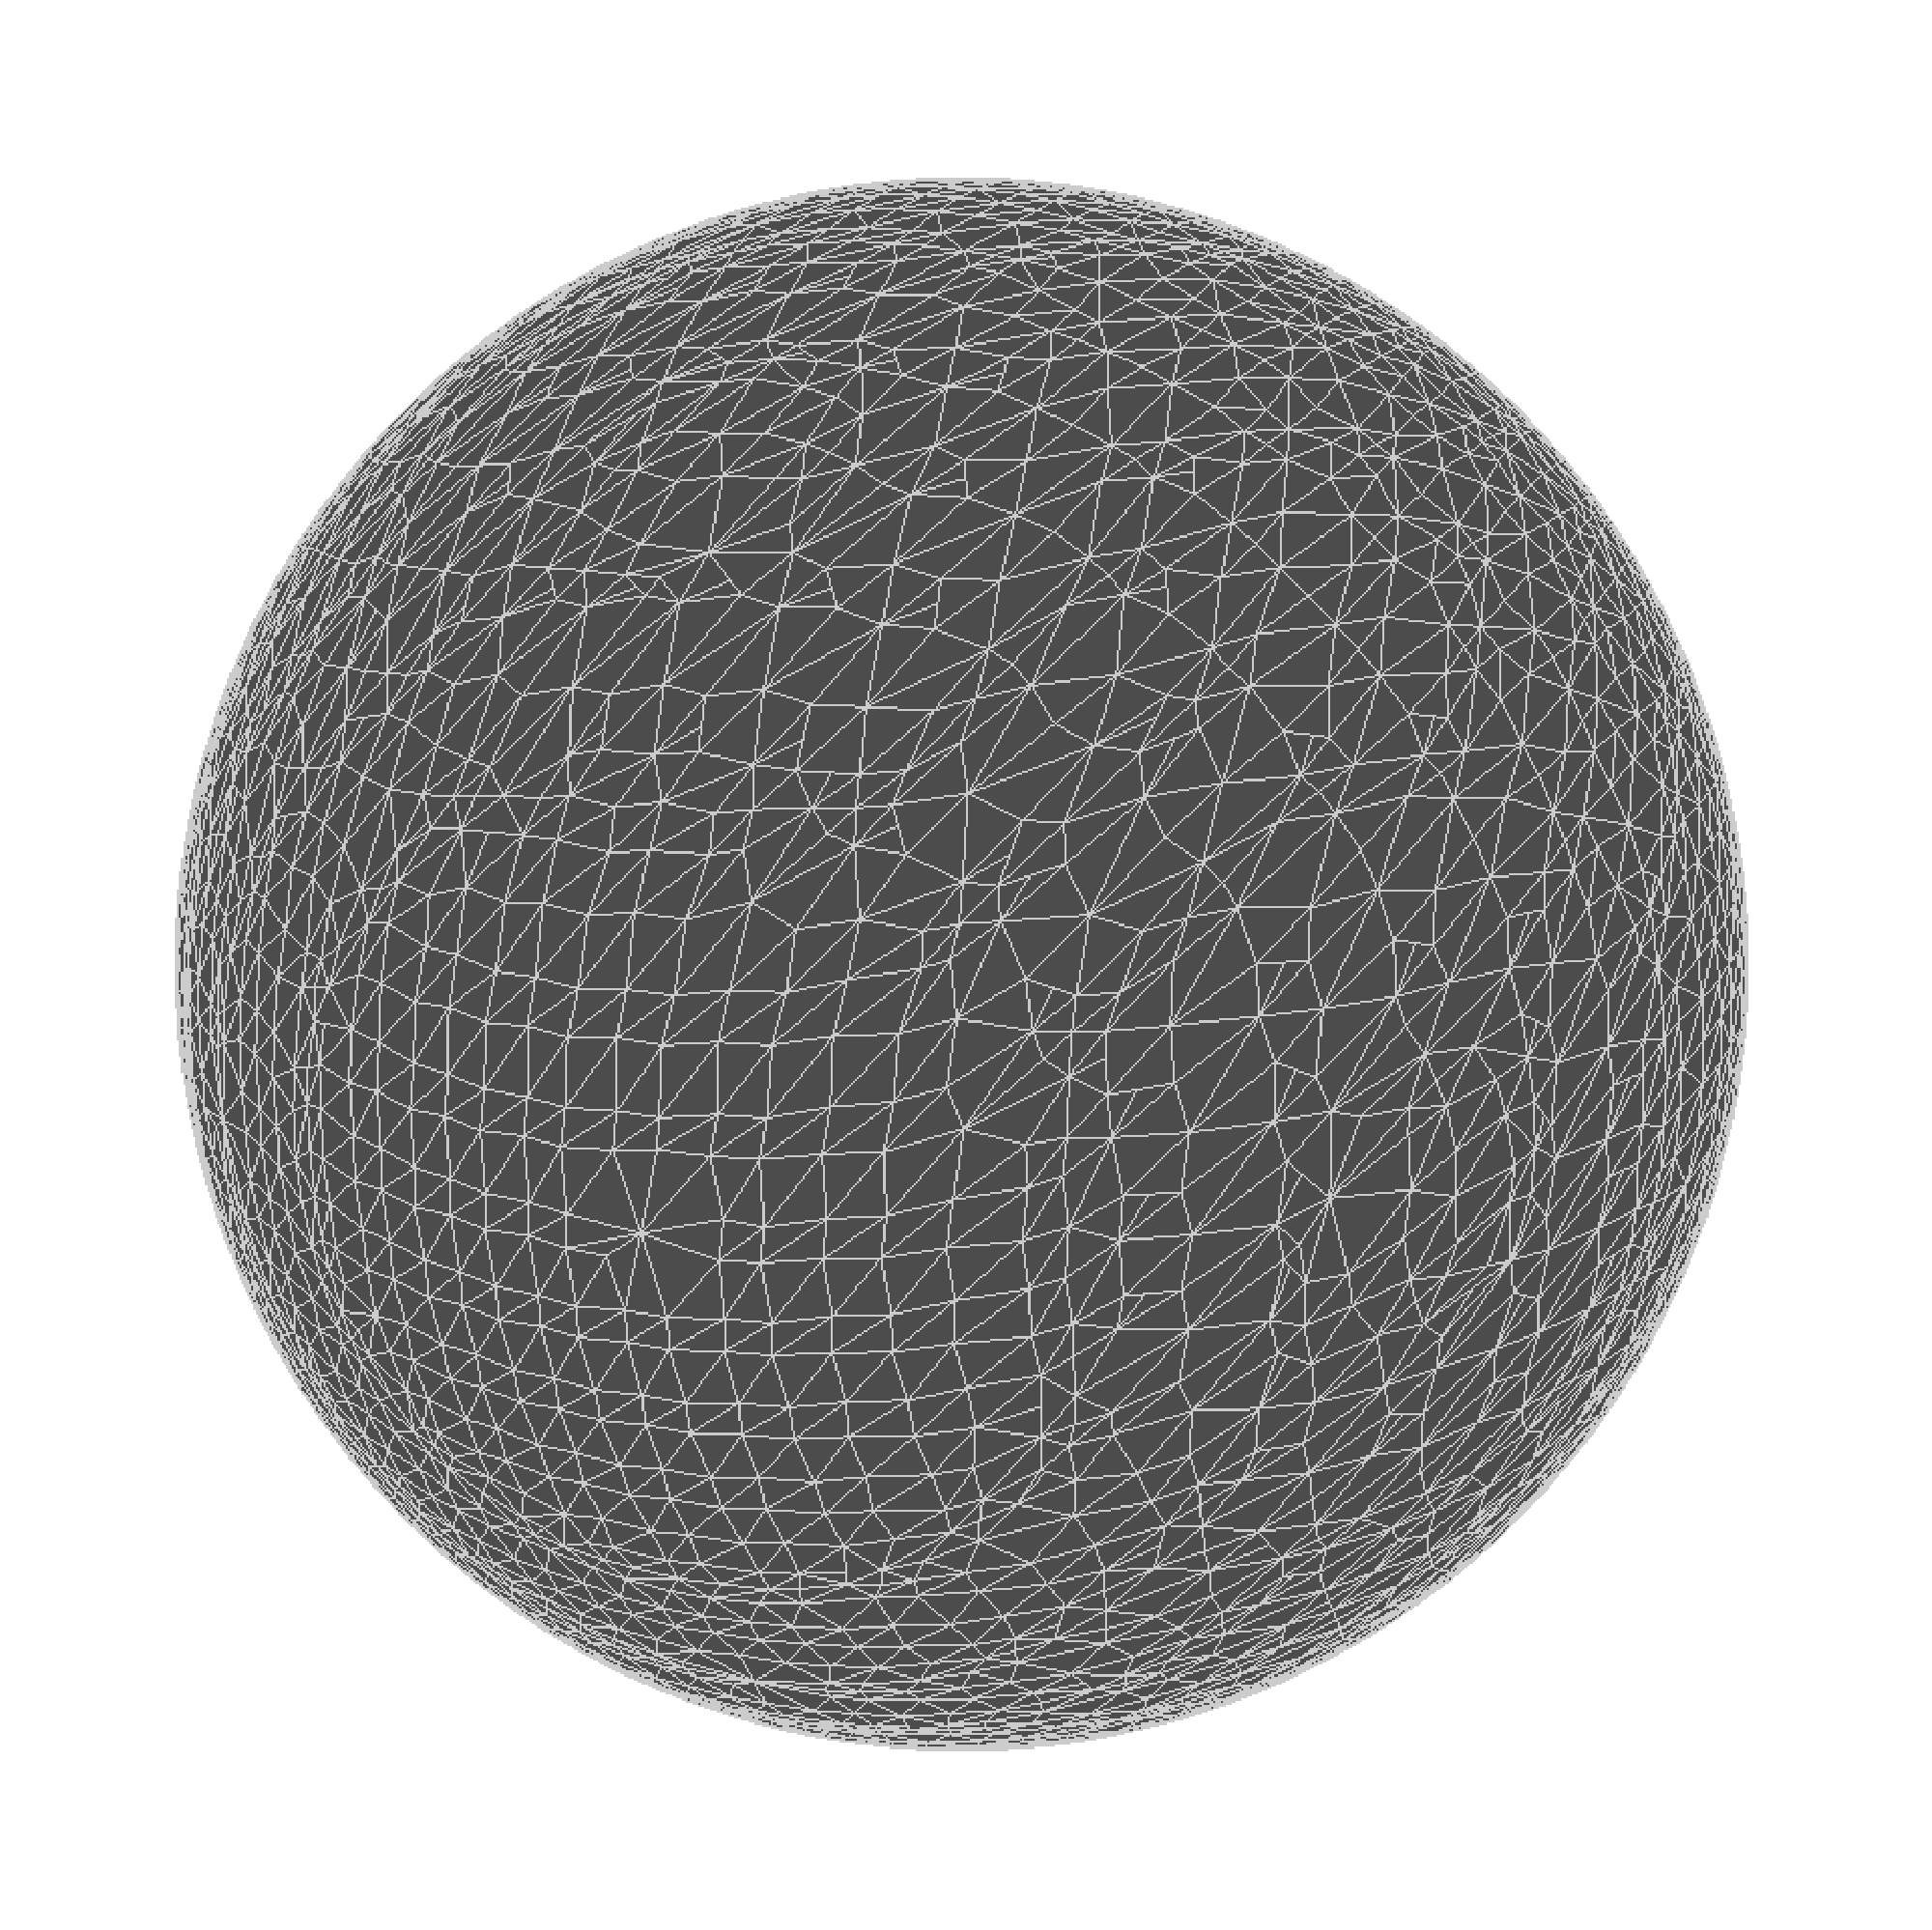
\includegraphics[width=\textwidth]{figures/10iter_sphere_mesh}
				\caption{10 iterações de suavização}				
			\end{subfigure}
			\begin{subfigure}[b]{0.45\textwidth}
				\centering
				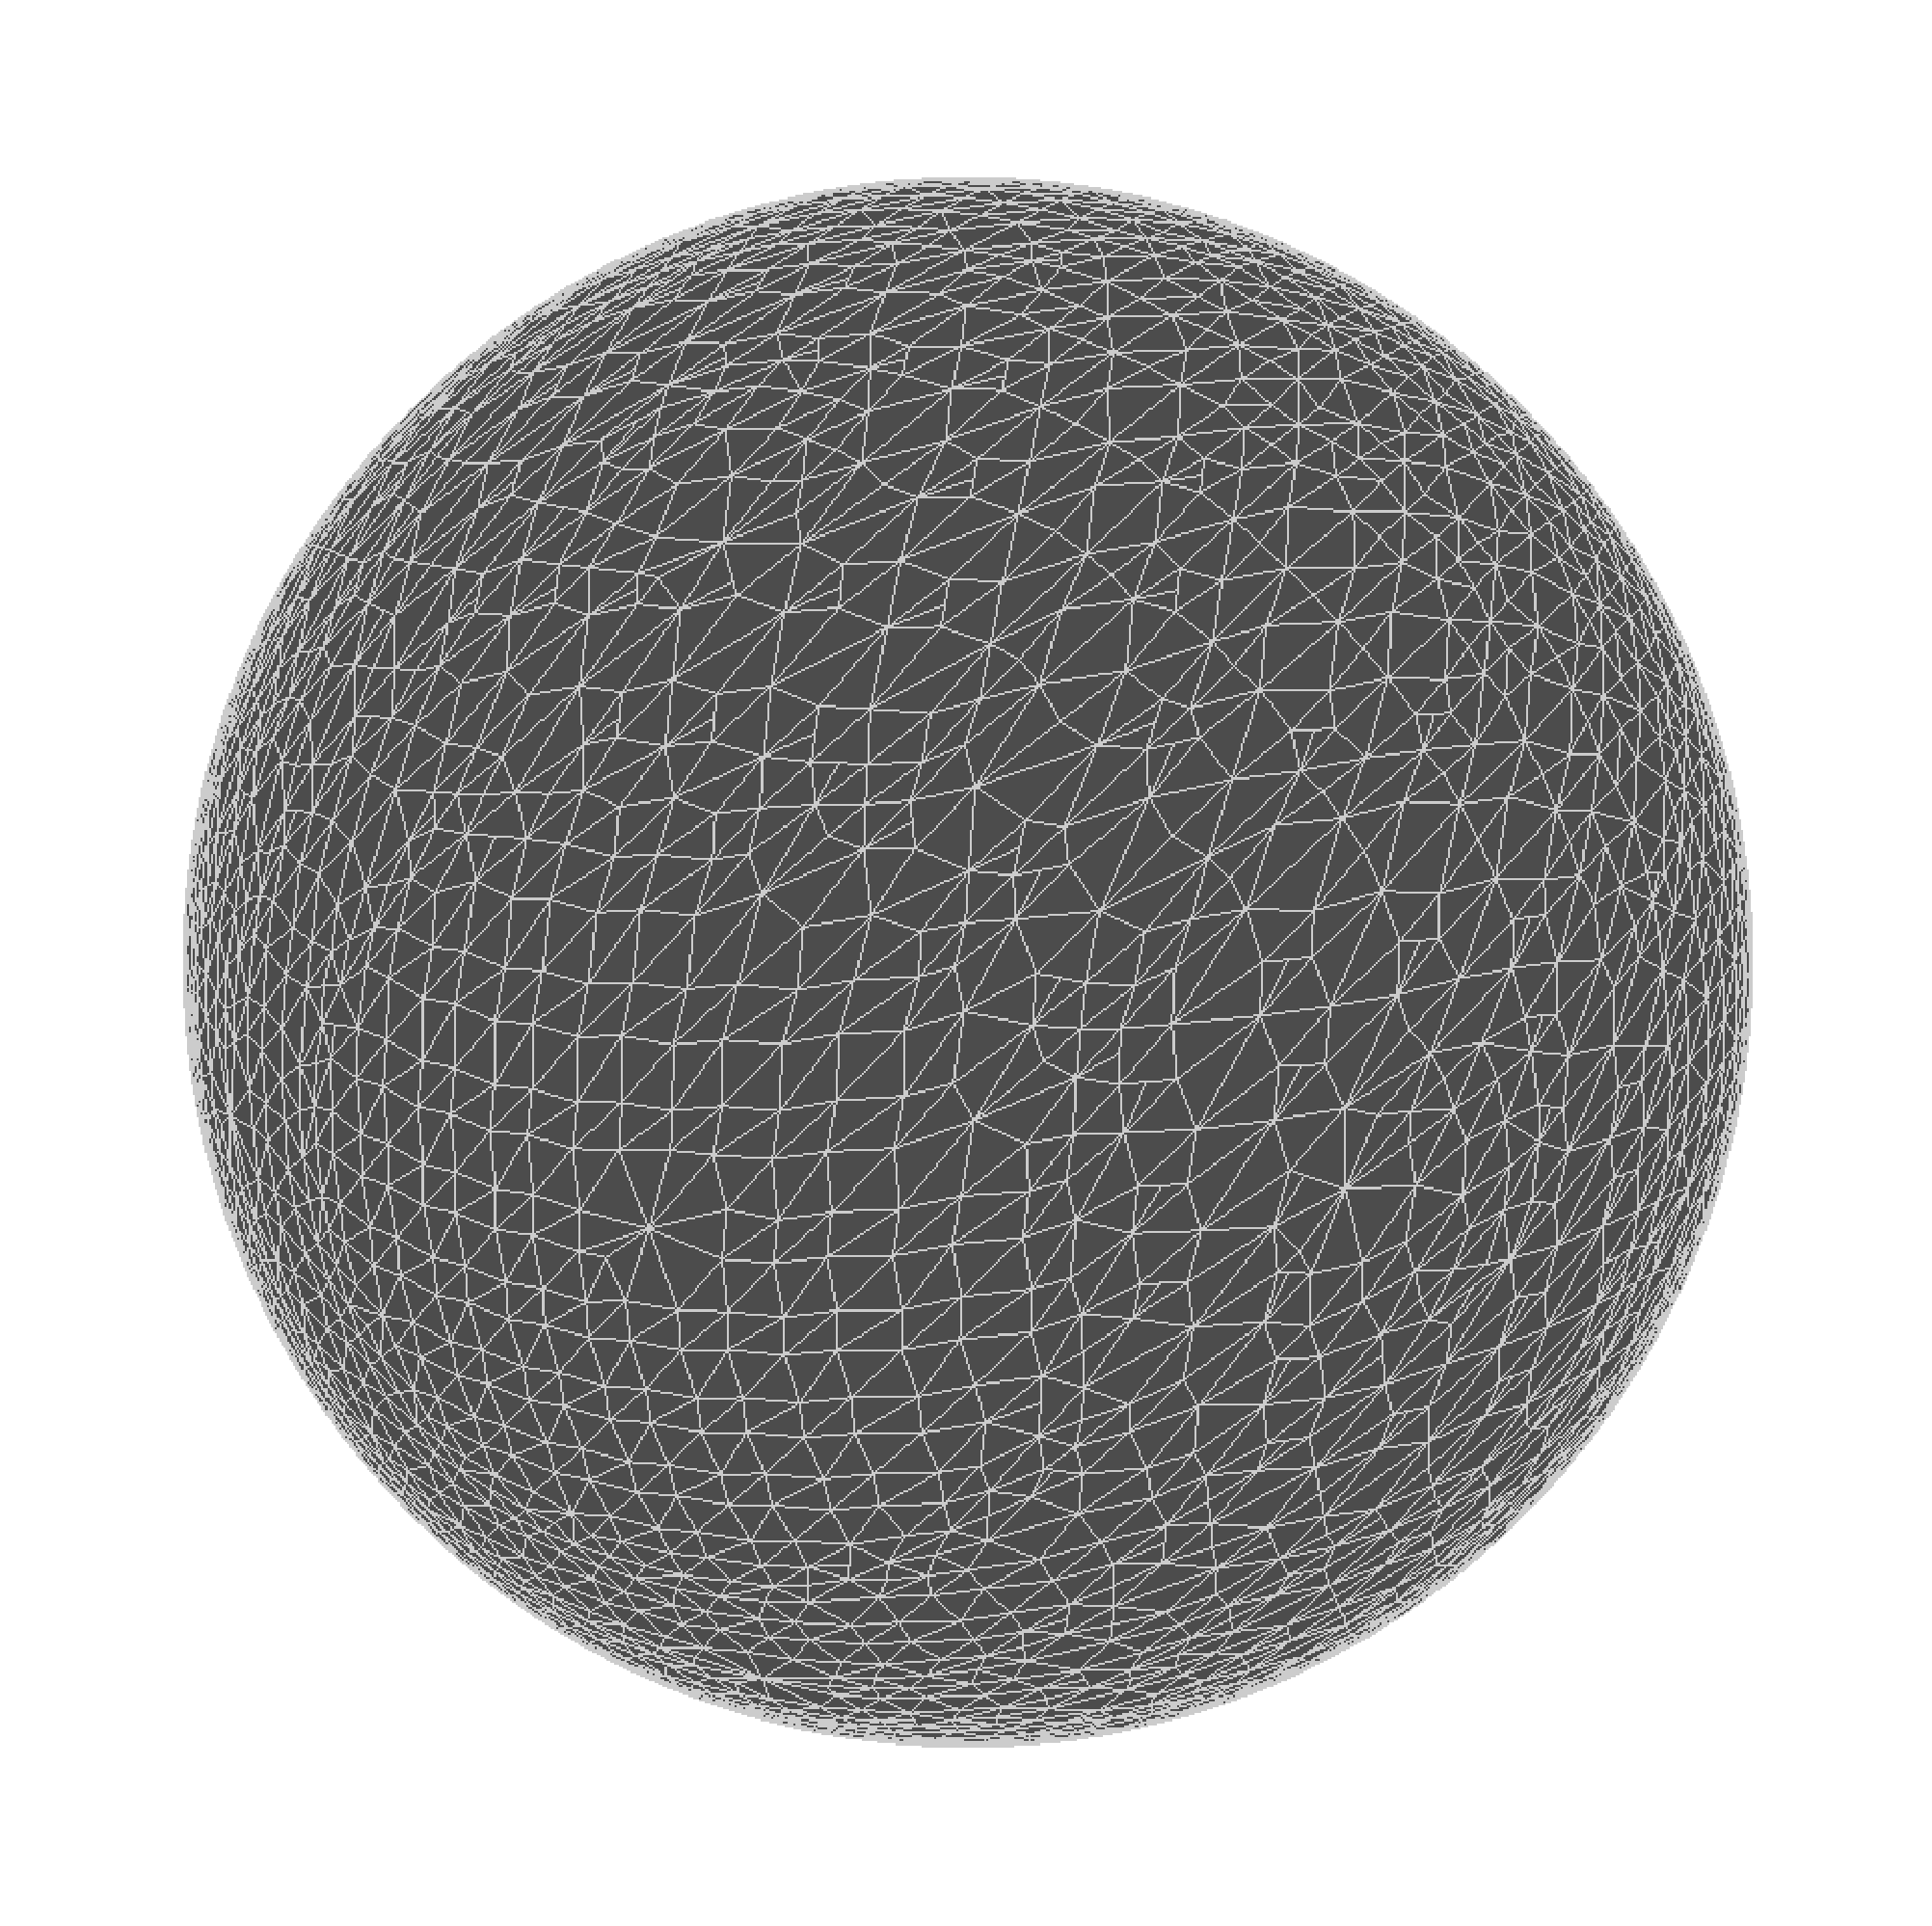
\includegraphics[width=\textwidth]{figures/20iter_sphere_mesh}
				\caption{20 iterações de suavização}				
			\end{subfigure}
			\begin{subfigure}[b]{0.45\textwidth}
				\centering
				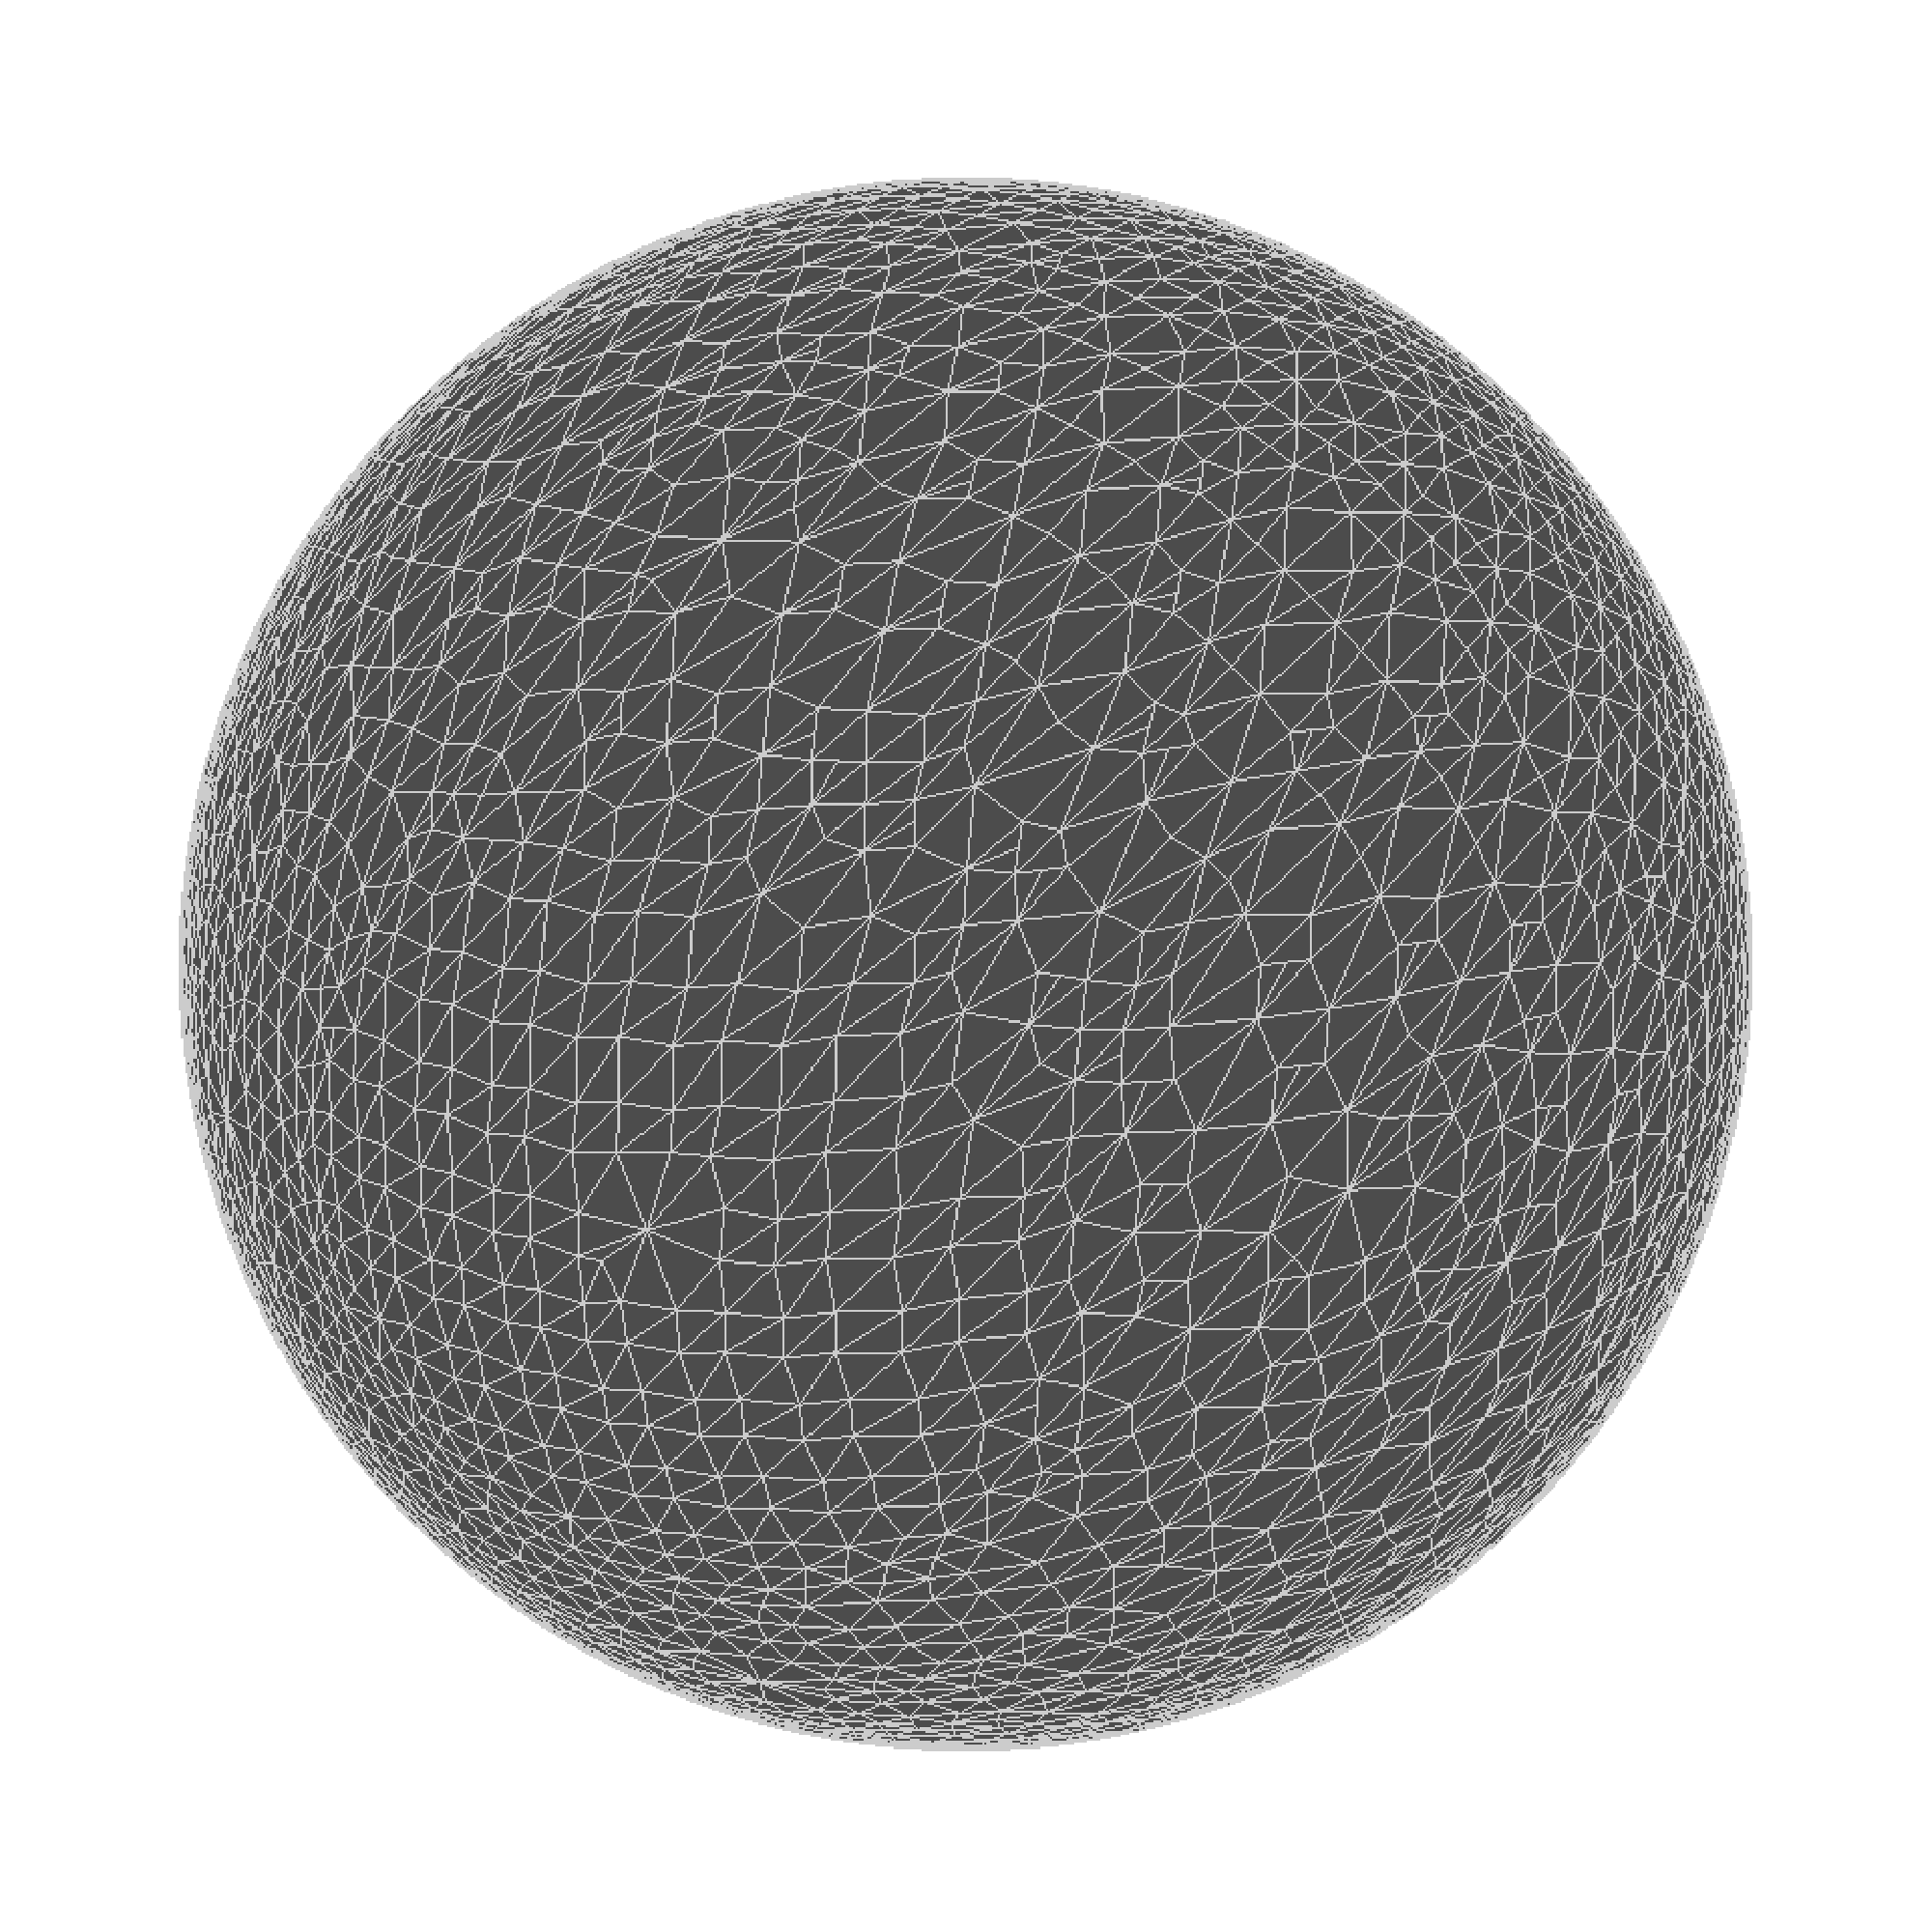
\includegraphics[width=\textwidth]{figures/30iter_sphere_mesh}
				\caption{30 iterações de suavização}				
			\end{subfigure}
			\caption{Malha de triângulos gerada para a esfera de raio 1}
			\label{fig:mesh:sphere}
		\end{figure}
		\begin{figure}
			\centering
			\begin{subfigure}[b]{0.45\textwidth}
				\centering
				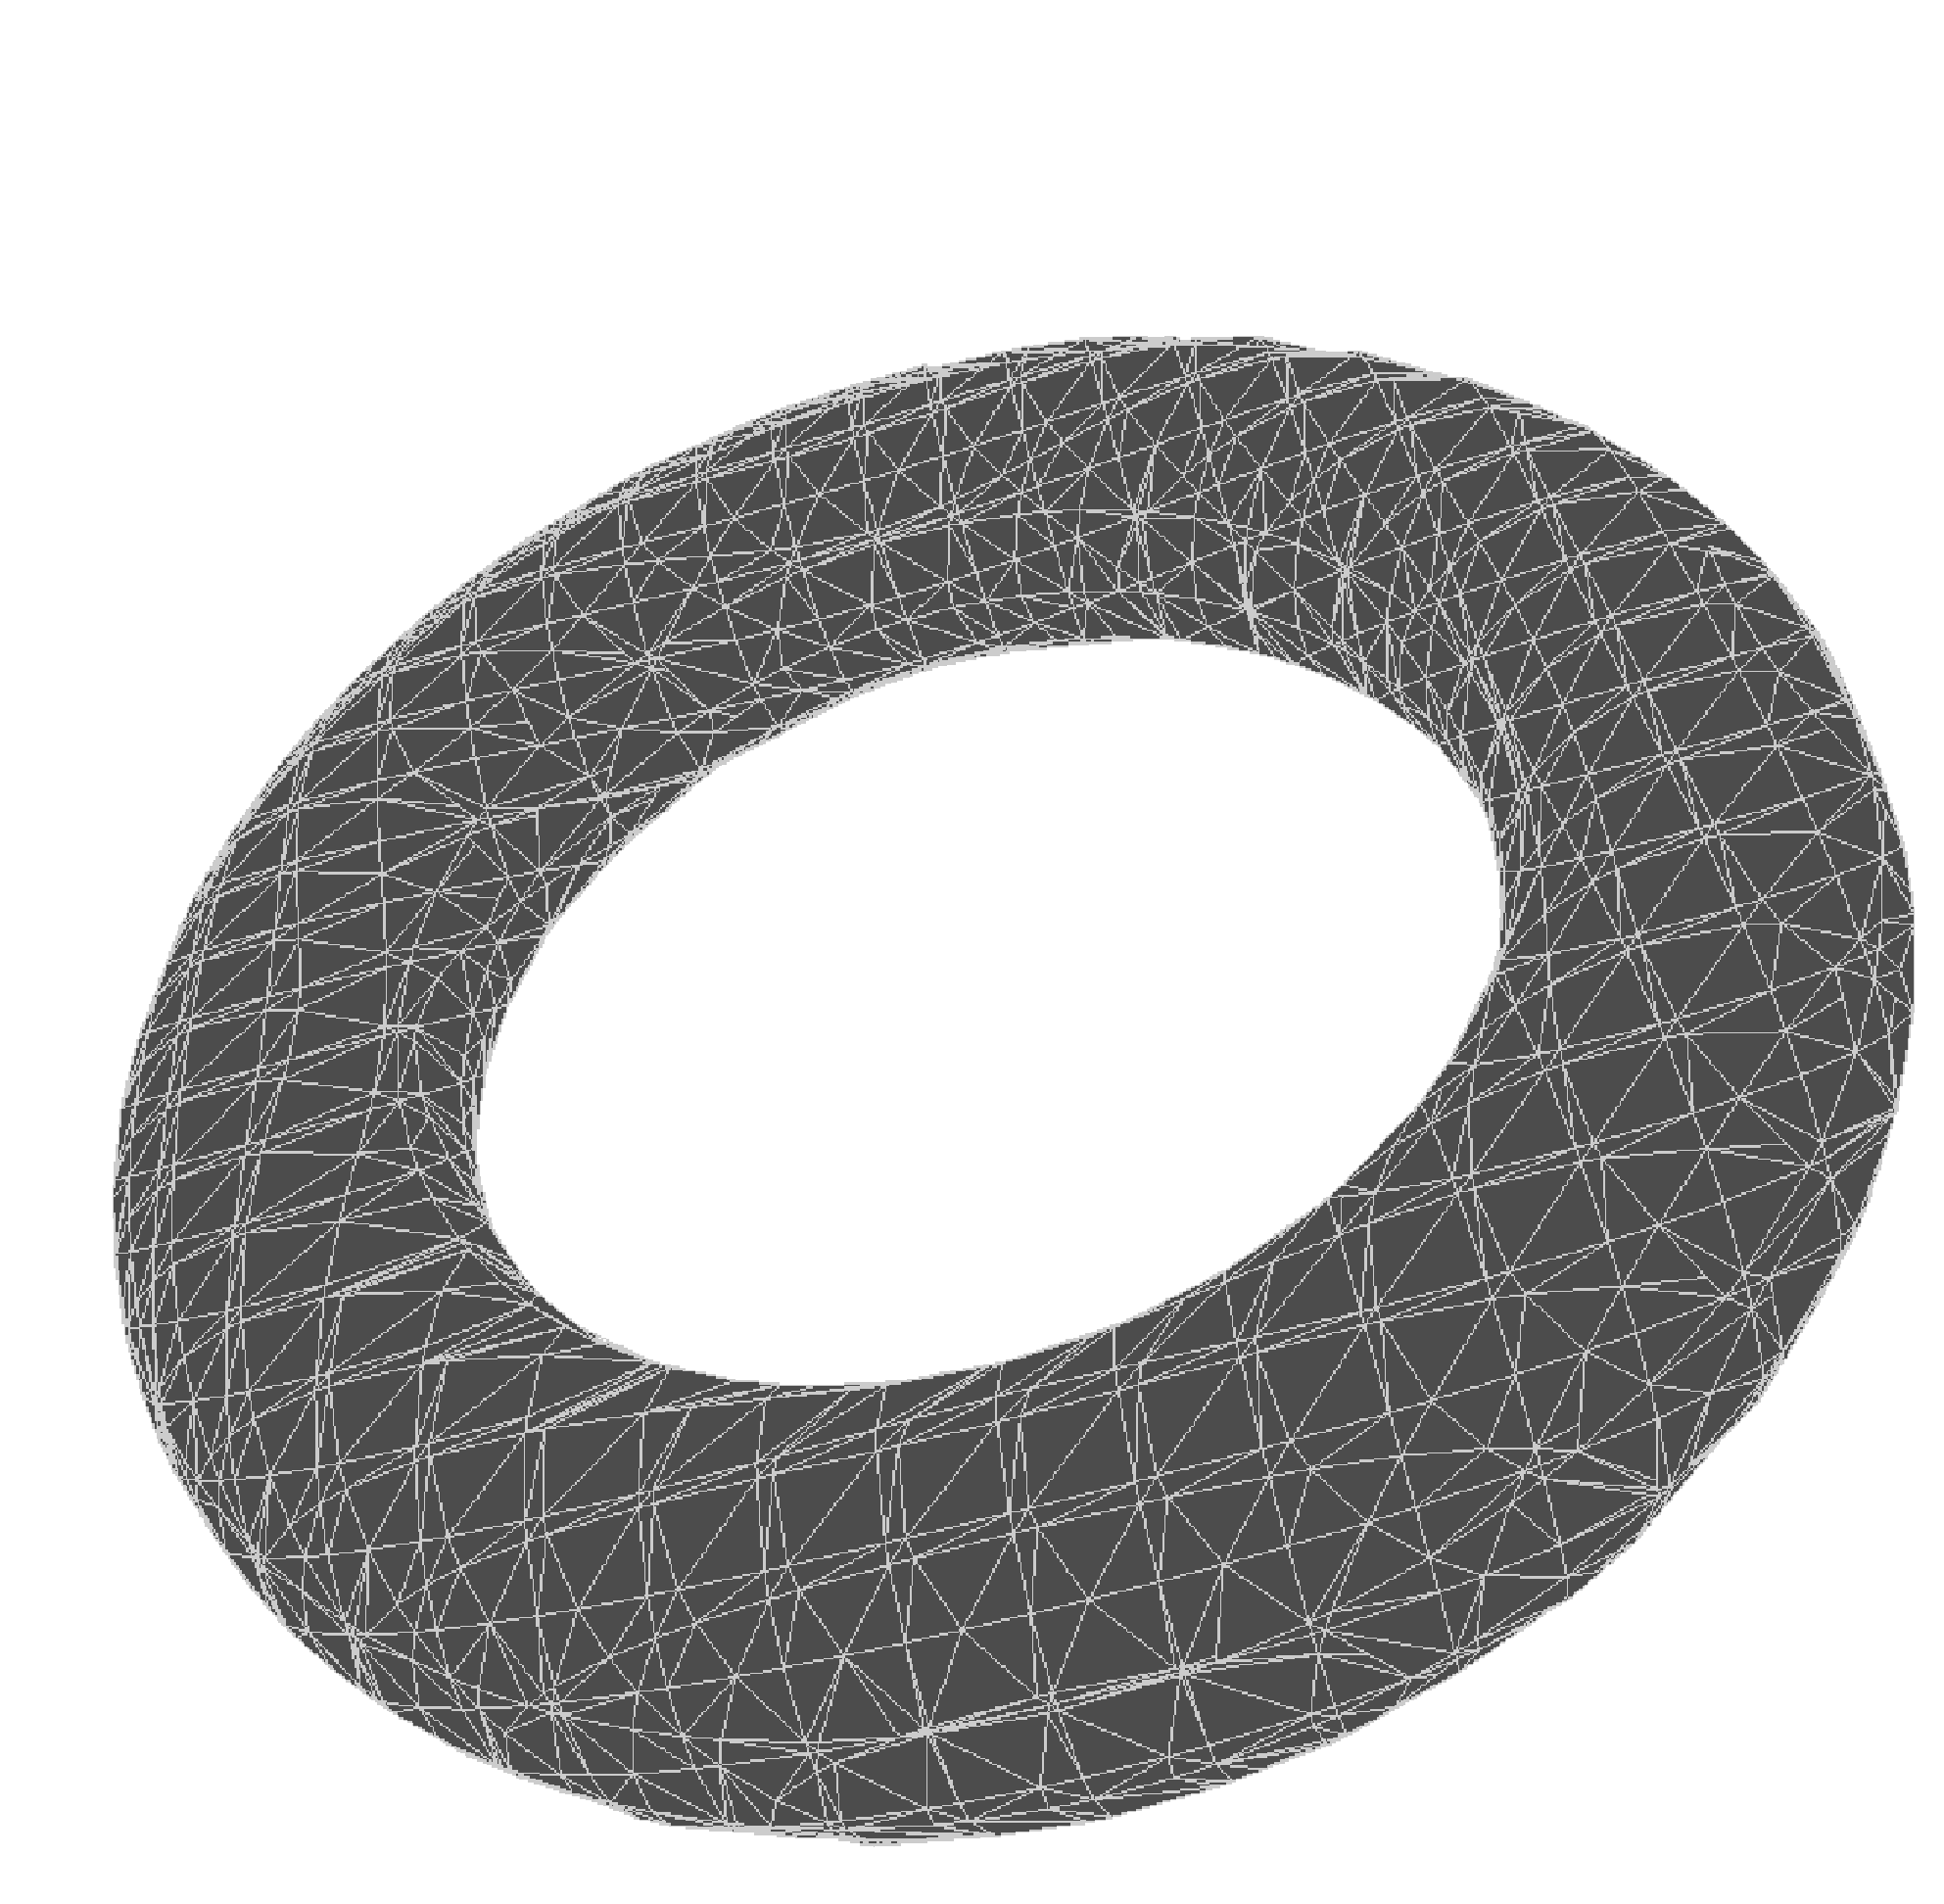
\includegraphics[width=\textwidth]{figures/0iter_torus_mesh}
				\caption{Malha inicial}				
			\end{subfigure}
			\begin{subfigure}[b]{0.45\textwidth}
				\centering
				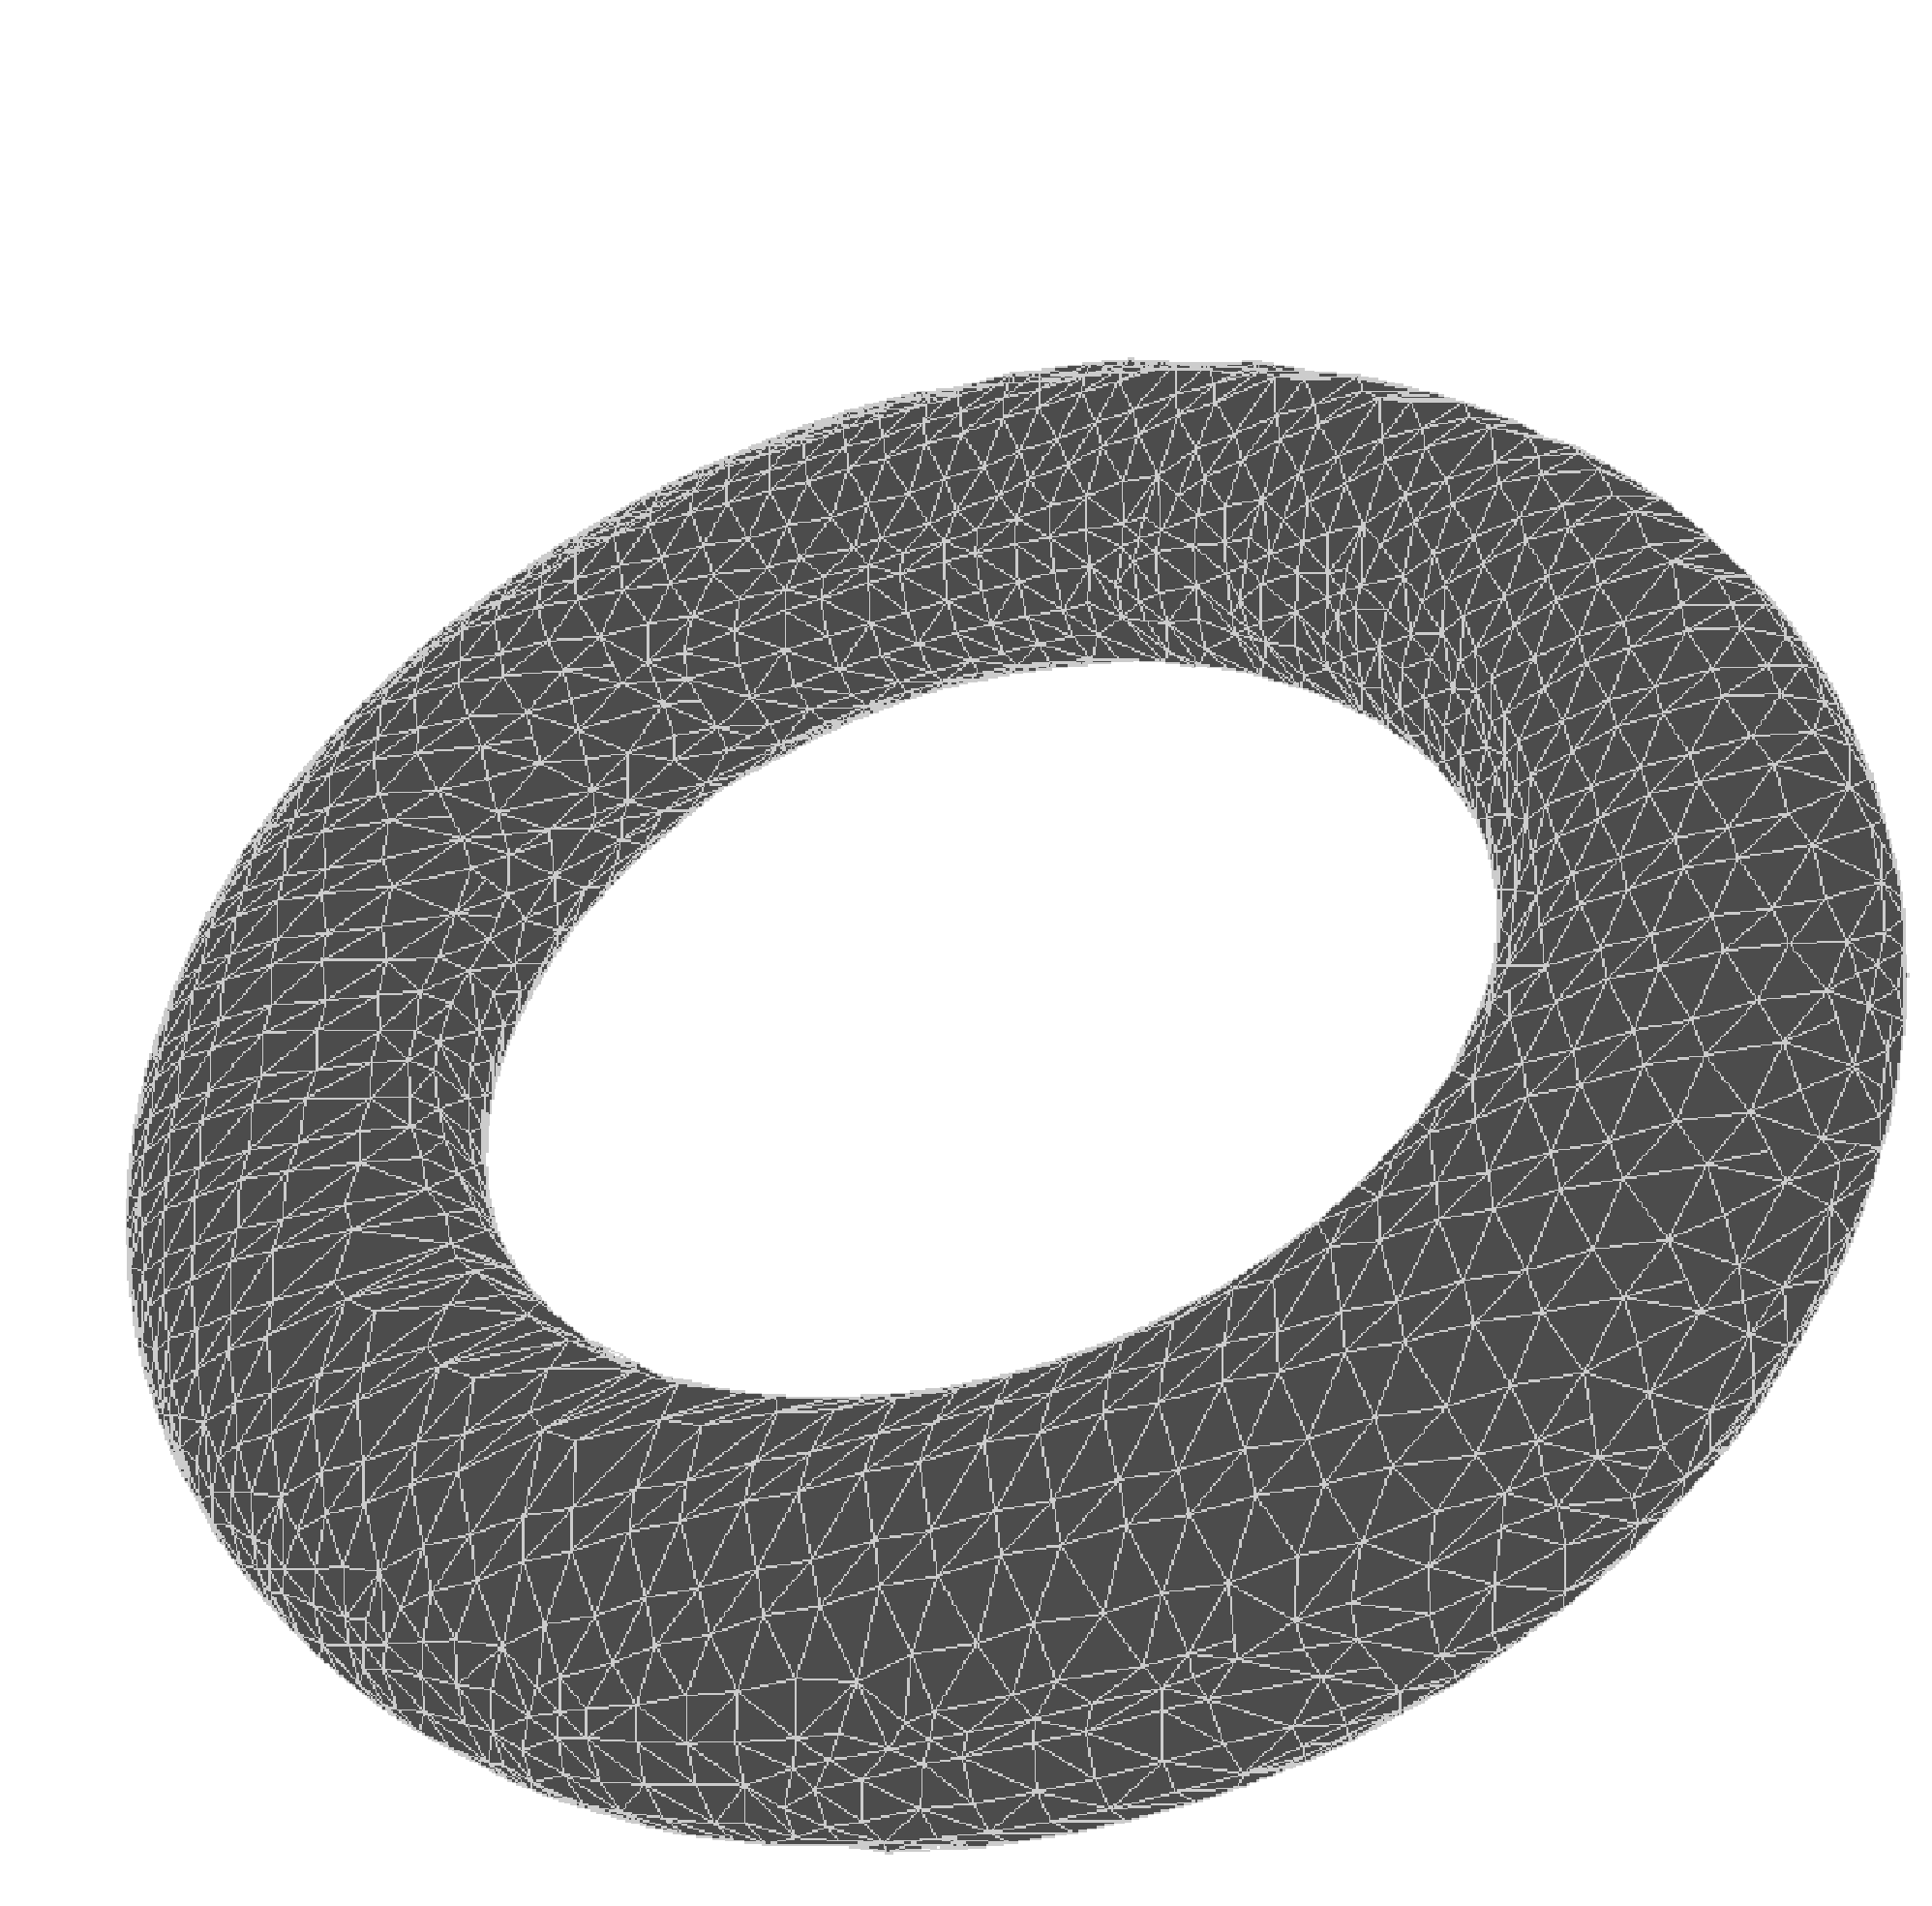
\includegraphics[width=\textwidth]{figures/10iter_torus_mesh}
				\caption{10 iterações de suavização}				
			\end{subfigure}
			\begin{subfigure}[b]{0.45\textwidth}
				\centering
				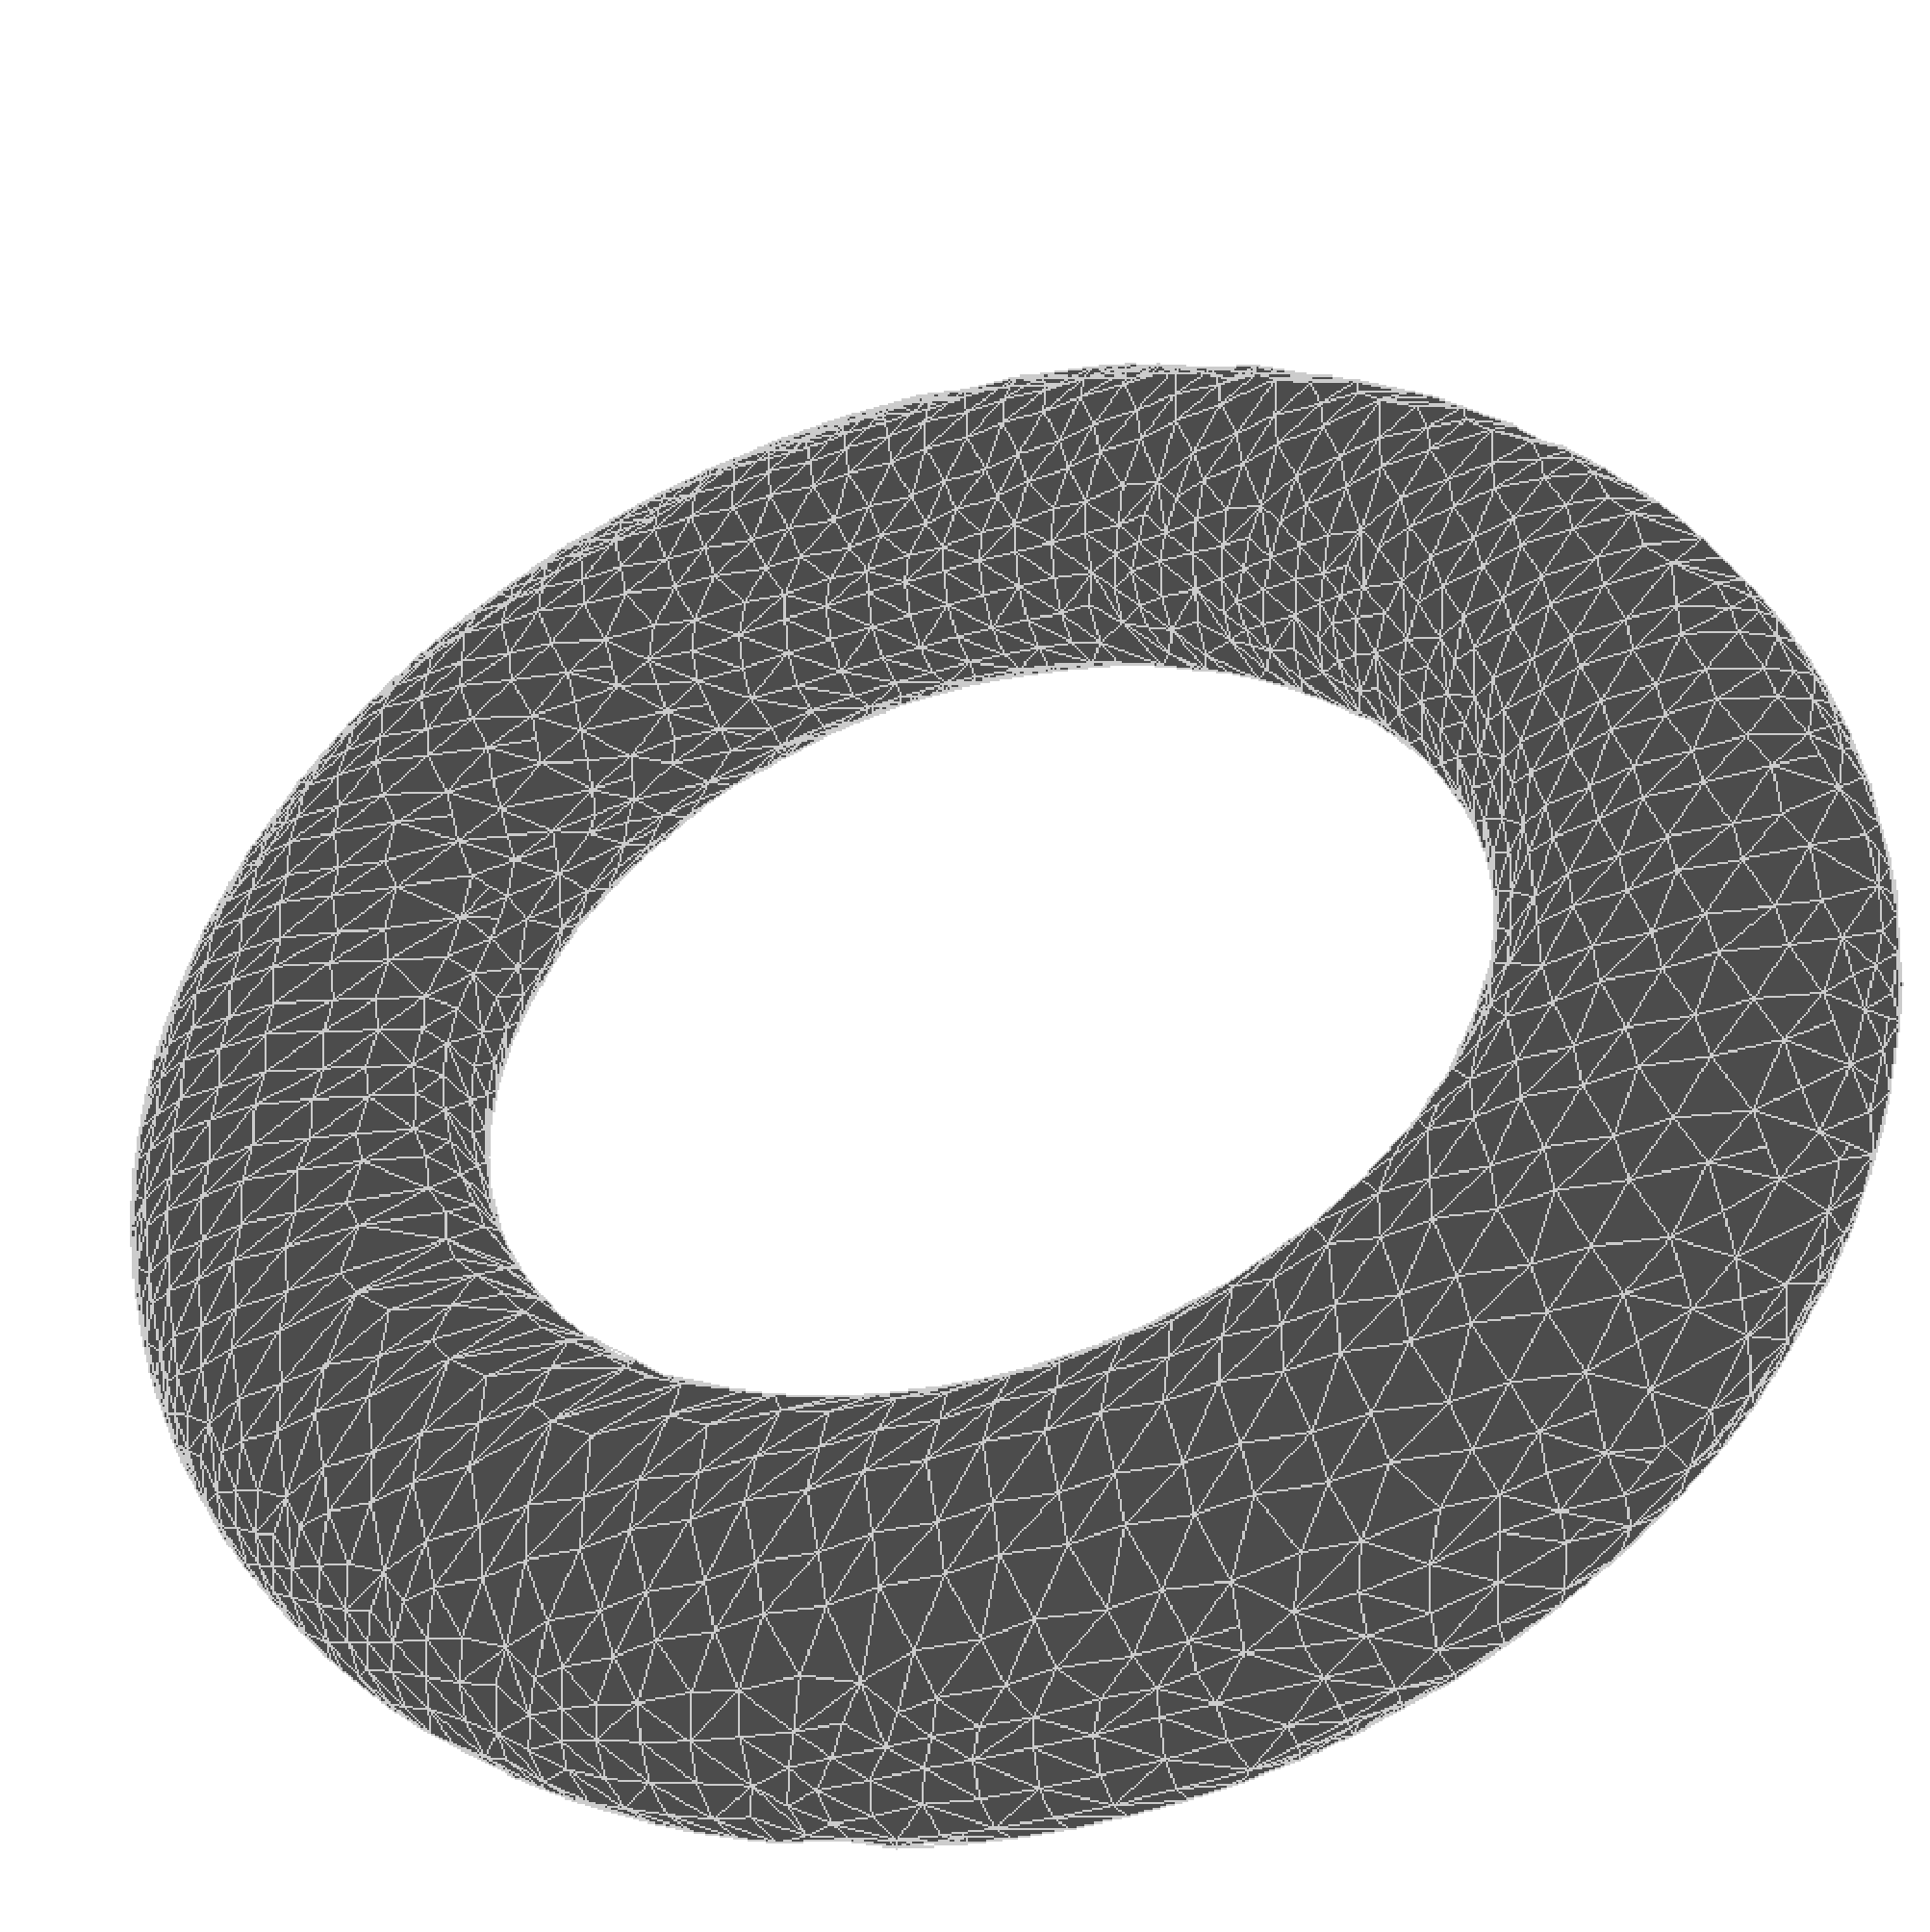
\includegraphics[width=\textwidth]{figures/20iter_torus_mesh}
				\caption{20 iterações de suavização}				
			\end{subfigure}
			\begin{subfigure}[b]{0.45\textwidth}
				\centering
				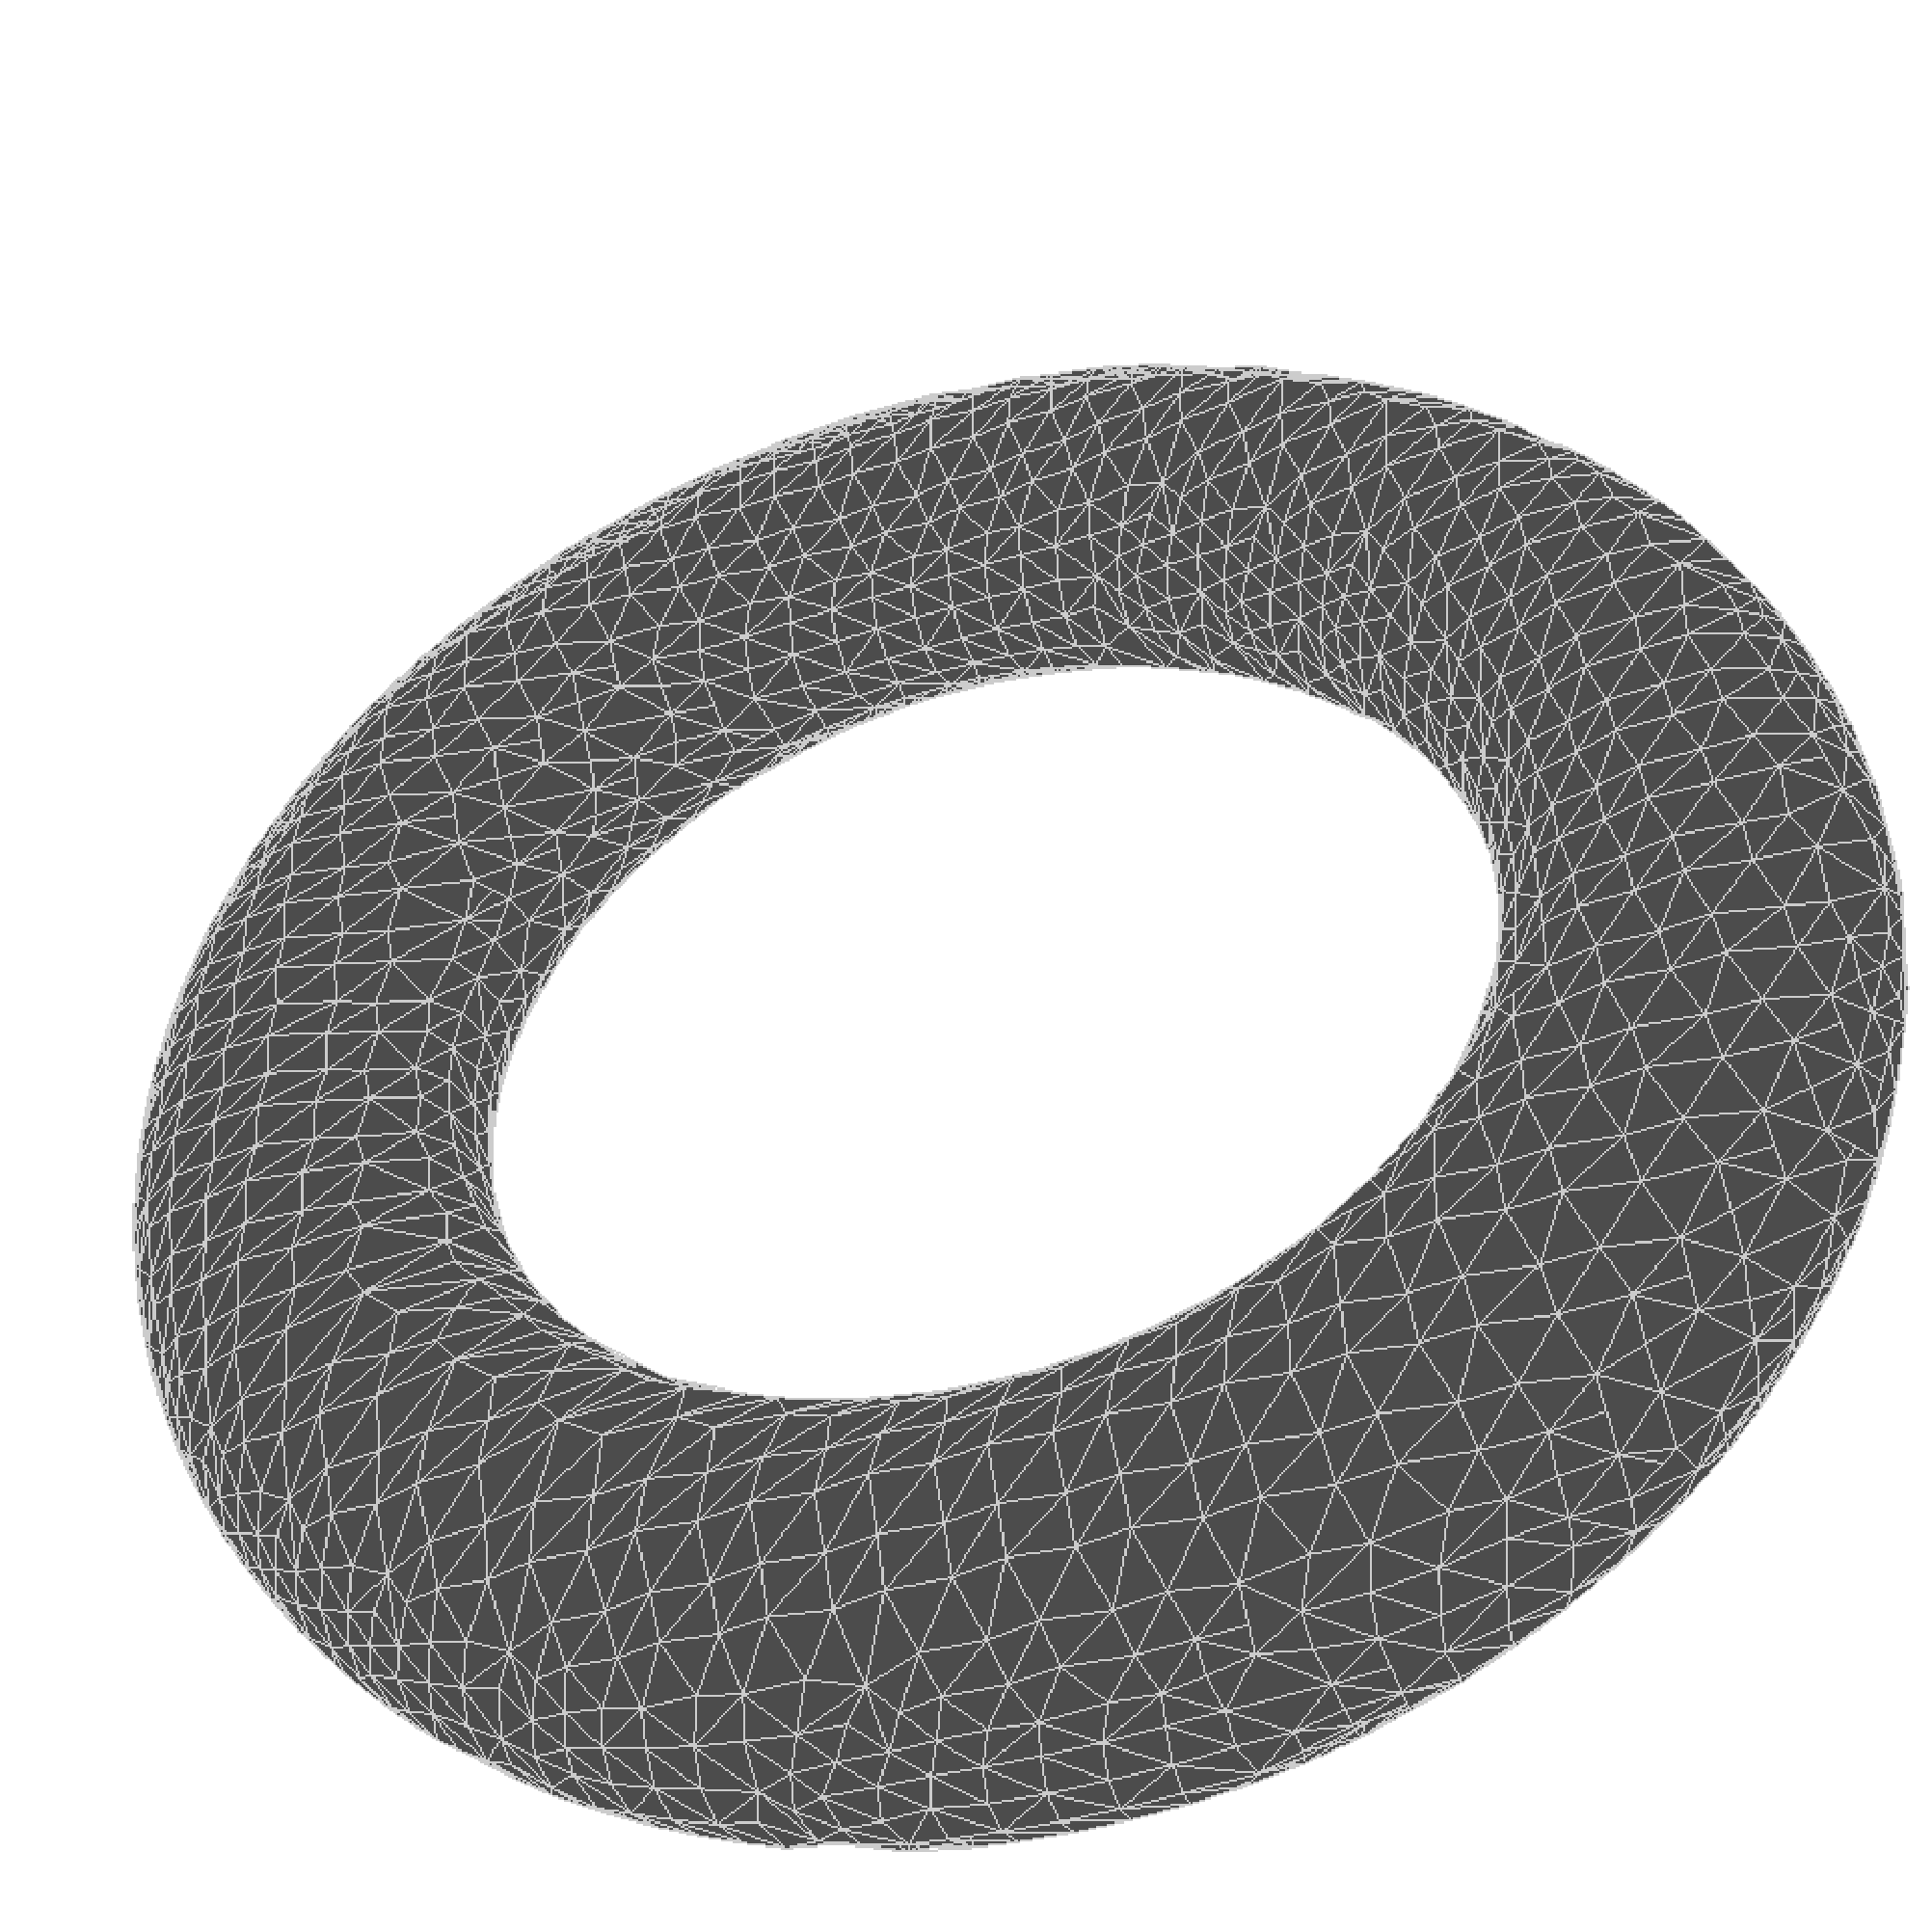
\includegraphics[width=\textwidth]{figures/30iter_torus_mesh}
				\caption{30 iterações de suavização}				
			\end{subfigure}
			\caption{Malha de triângulos gerada para o toro com raios 1 e 0.25}
			\label{fig:mesh:torus}
		\end{figure}

		%%%%%%%%%%%%%%%
		% Histogramas %
		%%%%%%%%%%%%%%%

		\begin{figure}
			\centering
			\begin{subfigure}[b]{0.45\textwidth}
				\centering
				\includegraphics[width=\textwidth]{figures/0iter_sphere}
				\caption{Qualidade inicial}				
			\end{subfigure}
			\begin{subfigure}[b]{0.45\textwidth}
				\centering
				\includegraphics[width=\textwidth]{figures/10iter_sphere}
				\caption{10 iterações de suavização}				
			\end{subfigure}
			\begin{subfigure}[b]{0.45\textwidth}
				\centering
				\includegraphics[width=\textwidth]{figures/20iter_sphere}
				\caption{20 iterações de suavização}				
			\end{subfigure}
			\begin{subfigure}[b]{0.45\textwidth}
				\centering
				\includegraphics[width=\textwidth]{figures/30iter_sphere}
				\caption{30 iterações de suavização}				
			\end{subfigure}
			\caption{Histogramasde qualidade dos triângulos para a esfera de raio 1}
			\label{fig:hist:sphere}
		\end{figure}
		\begin{figure}
			\centering
			\begin{subfigure}[b]{0.45\textwidth}
				\centering
				\includegraphics[width=\textwidth]{figures/0iter_torus}
				\caption{Qualidade inicial}				
			\end{subfigure}
			\begin{subfigure}[b]{0.45\textwidth}
				\centering
				\includegraphics[width=\textwidth]{figures/10iter_torus}
				\caption{10 iterações de suavização}				
			\end{subfigure}
			\begin{subfigure}[b]{0.45\textwidth}
				\centering
				\includegraphics[width=\textwidth]{figures/20iter_torus}
				\caption{20 iterações de suavização}				
			\end{subfigure}
			\begin{subfigure}[b]{0.45\textwidth}
				\centering
				\includegraphics[width=\textwidth]{figures/30iter_torus}
				\caption{30 iterações de suavização}				
			\end{subfigure}
			\caption{Histogramasde qualidade dos triângulos para o toro com raios 1 e 0.25}
			\label{fig:hist:torus}
		\end{figure}
	% section resultados (end)

	% \nocite{*}
	\bibliography{refs.bib}
	\bibliographystyle{acm}
\end{document}
